\documentclass[letterpaper, 10 pt, conference]{ieeeconf}  % Comment this line out
                                                          % if you need a4paper
%\documentclass[a4paper, 10pt, conference]{ieeeconf}      % Use this line for a4
                                                          % paper

\IEEEoverridecommandlockouts                              % This command is only
                                                          % needed if you want to
                                                          % use the \thanks command
\overrideIEEEmargins
% See the \addtolength command later in the file to balance the column lengths
% on the last page of the document



% The following packages can be found on http:\\www.ctan.org
%\usepackage{graphics} % for pdf, bitmapped graphics files
%\usepackage{epsfig} % for postscript graphics files
%\usepackage{mathptmx} % assumes new font selection scheme installed
%\usepackage{times} % assumes new font selection scheme installed
%\usepackage{amsmath} % assumes amsmath package installed
%\usepackage{amssymb}  % assumes amsmath package installed

\usepackage[prependcaption,textsize=tiny]{todonotes}
\usepackage{amssymb}
\usepackage{amsmath}
\usepackage{minted}
\usepackage{cite}
\usepackage[utf8]{inputenc}
\usepackage[gen]{eurosym}
\usepackage{etoolbox}


\usepackage{tikz-cd}
\usetikzlibrary{positioning}
\usetikzlibrary{fit}
\usetikzlibrary{cd}
\usetikzlibrary{arrows}
\usetikzlibrary{calc}
\usetikzlibrary{decorations.markings}
\tikzset{ed/.style={auto,inner sep=2pt,font=\scriptsize}} %edges
\tikzset{>=stealth'}
\tikzset{vert/.style={draw,circle, minimum size=6mm, inner sep=0pt, fill=white}}
\tikzset{vertbig/.style={draw,circle, minimum size=8mm, inner sep=0pt, fill=white}}
\tikzset{->-/.style={decoration={
      markings,
      mark=at position #1 with {\arrow{>}}},postaction={decorate}}}

\newtheorem{definition}{Definition}[paragraph]
\newcounter{snippet}
\setcounter{snippet}{1}
\newcommand{\Optic}{\textbf{Optic}}
\newcommand{\hto}{\ensuremath{\,\mathaccent\shortmid\rightarrow\,}}
\newcommand{\id}{\text{id}}
\newcommand{\R}{\mathbb{R}}
\newcommand{\Hom}{\text{Hom}}
\DeclareSymbolFont{bbsymbol}{U}{bbold}{m}{n}
\DeclareMathSymbol{\bbsemi}{\mathbin}{bbsymbol}{"3B}

\DeclareUnicodeCharacter{2032}{\ensuremath{^\prime}}
\DeclareUnicodeCharacter{2081}{\ensuremath{_1}}
\DeclareUnicodeCharacter{2082}{\ensuremath{_2}}
\DeclareUnicodeCharacter{2A1F}{\ensuremath{\bbsemi}}

\newenvironment{snippet}{
    \VerbatimEnvironment\begin{minted}[frame=lines,framesep=2mm,fontsize=\footnotesize, xleftmargin=0.5em, mathescape, linenos, label=Snippet \arabic{snippet}, labelposition=topline, escapeinside=||, mathescape=true]{julia}}{\end{minted}\addtocounter{snippet}{1}}

\title{\LARGE \bf
$\partial P$.jl\footnote{Working name} terminology and notation guide}

\author{Keno Fischer}

\begin{document}

\maketitle

\section*{Foreword}

The field of automatic differentiation (AD) has a long history, both in the academic
literature and in programming practice. However, despite this long history,
or perhaps because of it, the terminology for various concepts and operations
is neither standard nor consistent. This inconsistency imposes upon new
implementers of AD tools a burden to clearly state the
meaning of any terminology they might venture to employ. This document is an
attempt to do such that for my present work on a new AD
tool for the Julia language. It is intended 1) to give contributors and users a
common vocabulary to discuss the manifold abstractions required to create a
modern AD tools, 2) to explain why certain terminology may have been
chosen and 3) to serve implementers as a guide to the proper functioning of the
tool when lost deep in the web of details. By necessity, the terminology in
this guide is borrowed from several different fields of study (most relevantly
category theory and differential geometry). Nevertheless, this guide does not
intend to be an introduction to these fields, nor does it assume that readers
have had such an introduction. Instead, we try to give some examples and
intuition for why the abstractions chosen are of interest to the implementation
of automatic differentiation. Lastly, despite using terminology that might
be amenable to formalization, this document is not an attempt to do so and as
such certain liberties may be taken that would require careful treatment in a
more formal treatise. With that out of the way, let's begin:

\section{Optical Constructions}

To begin our quest, we shall first put aside the topic of differentiation
entirely and study a relatively recent construction from category theory known
as an \textit{optic}. The power of the optic construction
lies in its ability to combine both a covariant and a contravariant
transformation in one abstraction while retaining composability.
Following Riley~\cite{riley:optics}, we briefly consider the following
explicit description of an optic (those not familiar with the language
of category theory are encouraged to skip straight to the diagrams).

\begin{definition}
For some symmetric monoidal category $\mathcal{C}$, we define the category
$\Optic_{\mathcal{C}}$. Whose objects are pairs $(A, A')$ of objects in $\mathcal{C}$
and whose morphisms have representatives given by $\langle l | r \rangle: (A, A') \hto (B, B')$
are pairs $(l, r)$ where $l: A \to M \otimes B$, $r: M \otimes B' \to A'$ (the choice of the object $M$ depending
on the representative - see Riley for details).
\end{definition}

This definition makes maniffest the combination of co- and contravariant data.
For a representative $\langle l | r \rangle$, $l$ varies covariantly while $r$
varies contravariantly. We additionally have a "memory" or "residual" object $M$.
This object is not uniquely determined and in fact we shall make good use of that
fact in our actual use case later. For now, We briefly exhibit the composition rules for these
morphisms. Suppose $\langle l_1 | r_1 \rangle: (A, A') \hto (B, B')$,
$\langle l_2 | r_2 \rangle: (B, B') \hto (C, C')$. Then
the sequenial composition $\langle l_{12} | r_{12} \rangle = \langle l_1 | r_1 \rangle \bbsemi \langle l_2 | r_2 \rangle$
may be written explicitly as

\[
l_{12}(a) := (m_1 \otimes m_2, c) \text { where } (m_1, b) = l_1(a), (m_2, c) = l_2(b) \]\[
r_{12}(m_1 \otimes m_2, c') := r_1(m_1, r_2(m_2, c'))
\]

While these definitions are perfectly explicit, it might be easier to understand
what is going on by considering optics diagramatically (diagrams taken from Riley\cite{riley:optics}).
For $\langle l | r \rangle$ we draw:

\begin{equation}
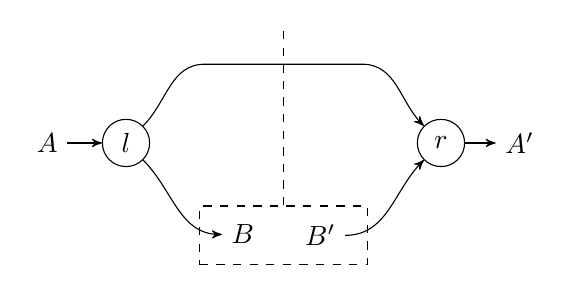
\begin{tikzpicture}[baseline=(S)]
    \node[vert] (l) at (0, 0) {$l$};
    \node[vert] (r) at (4, 0) {$r$};

    \node (S) [left of=l] {$A$};
    \node (A) [below right = 0.7 and 1 of l] {$B$};
    \node (S') [right of=r] {$A'$};
    \node (A') [below left = 0.7 and 1 of r] {$B'$};

    \draw[->] (S) -- (l);
    \draw[->] (l) to[out=south east,in=west] (A);

    \draw[<-] (S') -- (r);
    \draw[<-] (r) to[out=south west,in=east] (A');

    \draw[->] (l) to[out=north east, in=west] ++(1,1)
     to ++(2,0)
     to[out=east, in=north west] (r)
    ;

    \node[draw,dashed,fit=(A) (A'), inner xsep = 8pt] (box) {};
    \draw[dashed] (box.90) -- +(0,2.25);
\end{tikzpicture}
\end{equation}

We compose these optics by inserting one optic in the hole of another, e.g.
for the composition we have above, we might write
$\langle l_1 | r_1 \rangle \bbsemi \langle l_2 | r_2 \rangle$

\begin{equation}
    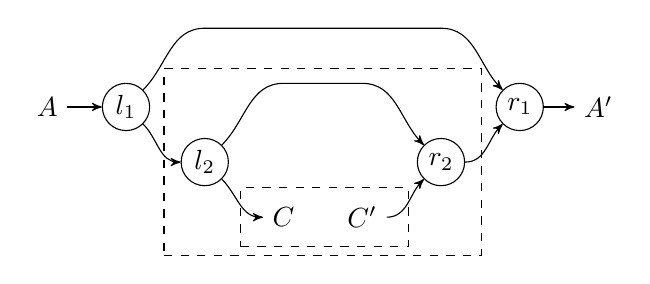
\begin{tikzpicture}[baseline=(R)]
        \begin{scope}[on grid]

        \node[vert] (l') at (0, 0) {$l_1$};
        \node[vert, below right = 0.7 and 1 of l'] (l) {$l_2$};
        \node[vert] (r') at (5, 0) {$r_1$};
        \node[vert, below left = 0.7 and 1 of r'] (r) {$r_2$};

        \node (A) [below right = 0.7 and 1 of l] {$C$};
        \node (A') [below left = 0.7 and 1 of r] {$C'$};

        \node (R) [left of=l'] {$A$};
        \node (R') [right of=r'] {$A'$};

        \draw[->] (R) -- (l');
        \draw[<-] (R') -- (r');

        \draw[->] (l') to[out=north east, in=west] ++(1,1)
         to ++(3,0)
         to[out=east, in=north west] (r')
        ;

        \draw[->] (l) to[out=north east, in=west] ++(1,1)
         to ++(1,0)
         to[out=east, in=north west] (r)
        ;

        \draw[->] (l') to[out=south east,in=west] (l);
        \draw[->] (r) to[out=east, in=south west] (r');

        \draw[->] (l) to[out=south east,in=west] (A);
        \draw[<-] (r) to[out=south west,in=east] (A');

        \node[draw,dashed,fit=(l) (r), inner xsep = 6pt, inner ysep = 25pt] (box2) {};
        \node[draw,dashed,fit=(A) (A'), inner xsep = 8pt] (box) {};
        \end{scope}
        \end{tikzpicture}
\end{equation}

From the diagrammatic view, it is immediately clear that this composition
is indeed another optic and what the composition rule for these optics should
be:

\begin{equation}
    \begin{tikzpicture}[baseline=(R)]
        \begin{scope}[on grid]

        \node[vert] (l_1) at (0, 0) {};
        \node[vert, below right = 0.7 and 1 of l'] (l_2) {};
        \node[vert] (r_1) at (5, 0) {};
        \node[vert, below left = 0.7 and 1 of r'] (r_2) {};

        \node (C) [below right = 0.7 and 1 of l] {$C$};
        \node (C') [below left = 0.7 and 1 of r] {$C'$};

        \node (R) [left of=l'] {$A$};
        \node (R') [right of=r'] {$A'$};

        \draw[->] (R) -- (l');
        \draw[<-] (R') -- (r');

        \draw[->] (l') to[out=north east, in=west] ++(1,1)
         to ++(3,0)
         to[out=east, in=north west] (r')
        ;

        \draw[->] (l) to[out=north east, in=west] ++(1,1)
         to ++(1,0)
         to[out=east, in=north west] (r)
        ;

        \draw[->] (l') to[out=south east,in=west] (l);
        \draw[->] (r) to[out=east, in=south west] (r');

        \draw[->] (l) to[out=south east,in=west] (A);
        \draw[<-] (r) to[out=south west,in=east] (A');

        \node[circle,draw,dashed,fit=(l_1) (l_2), inner sep = 1pt, label=110:$l_{12}$] (l_12) {};
        \node[circle,draw,dashed,fit=(r_1) (r_2), inner sep = 1pt, label=80:$r_{12}$] (r_12) {};
        \node[draw,dashed,fit=(C) (C'), inner xsep = 8pt] (box) {};
        \end{scope}
        \end{tikzpicture}
\end{equation}

The reader is encouraged to verify that this diagrammatic derivation of $l_{12}$
and $r_{12}$ matches the algebraic definition above.

\subsection{Encoding Optics in Julia}

One of the original applications of optic constructions is the manipulation
of deeply nested data structures, so let's take that example and consider how
we might represent it in Julia. Optics for this application are often called
\textit{lenses}, though since we are just using them an an example here we shall
not concern ourselves with a precise definition. We begin by defining an
abstract optic type as well as a concrete representation of morphisms as pairs
$\langle l | r \rangle$:

\inputminted[frame=lines,framesep=2mm,fontsize=\footnotesize, xleftmargin=0.5em, mathescape, linenos, label={Snippet \arabic{snippet}}, labelposition=topline]{julia}{opticdef.jl}
\addtocounter{snippet}{1}

Given these definitions, we can now define an optic constructor that allows us
to modify an immutable value at a given location:

\begin{snippet}
SetIndex(idx) = OpticRepr(
    obj->(obj, getindex(obj, idx)),
    (obj, update)->setindex(obj, update, idx)
)
\end{snippet}

which we may use like so:

\begin{minted}[fontsize=\footnotesize,framesep=2mm]{julia}
julia> tup = (1,(2,3))
julia> o = SetIndex(2) ⨟ SetIndex(1)
julia> m, c = left(o, tup)
julia> c
2
julia> right(o, m, c + 100)
(1, (102, 3))
\end{minted}

However, as written, this definition as a big problem: It gives us the state `m`
explicitly. The type and value of `m` depends on the representative of the optic,
but nothing in our above definition requires the state `m` to be matched to the
optic representative `o`. To see the representation problem explicitly, suppose
we noticed that the state in this representation is somewhat suboptimal:

\begin{minted}[fontsize=\footnotesize,framesep=2mm]{julia}
julia> m
((1, (2, 3)), (2, 3))
\end{minted}

and instead defined a more optimized representation of the same optic:

\inputminted[frame=lines,framesep=2mm,fontsize=\footnotesize, xleftmargin=0.5em, mathescape, linenos, label={Snippet \arabic{snippet}}, labelposition=topline]{julia}{fastsetindex.jl}
\addtocounter{snippet}{1}

Our example from above goes through just the same:

\begin{minted}[fontsize=\footnotesize,framesep=2mm]{julia}
julia> tup = (1,(2,3))
julia> of = FastSetIndex(2) ⨟ FastSetIndex(1)
julia> m, c = left(of, tup)
julia> c
2
julia> right(of, m, c + 100)
(1, (102, 3))
\end{minted}

but our state is much smaller:

\begin{minted}[fontsize=\footnotesize,framesep=2mm]{julia}
julia> m
(1, (2, 3))
\end{minted}

With these two different representatives for the same optic, the
representative, dependence of `m` becomes quite apparent:

\begin{minted}[fontsize=\footnotesize,framesep=2mm]{julia}
julia> right(of, m, c + 100)
(1, (102, 3))

julia> right(o, m, c + 100)
ERROR: MethodError: no method matching
setindex(::Int64, ::Tuple{Int64,Int64}, ::Int64)
\end{minted}

In this example, this might be quite silly, but in general it presents a
problem depending on how the representative is chosen. E.g. an optic constructor
might perform a randomized search for the most efficient representative, so two
calls to the constructor will not necessarily yield the same representative. We
would thus prefer to have an interface to our optics that either does not
explicitly expose the state to the user, or if it does, tags the state with
a particular choice or representative. Here are two (equivalent) interfaces to
optics that have this property:

\inputminted[frame=lines,framesep=2mm,fontsize=\footnotesize, xleftmargin=0.5em, mathescape, linenos, label={Snippet \arabic{snippet}}, labelposition=topline]{julia}{opticcall.jl}

With these definitions, our update operation from above becomes

\begin{minted}[fontsize=\footnotesize,framesep=2mm]{julia}
julia> of(tup) do c
    c + 100
end
(1, (102, 3))

julia> c, back = of(tup);

julia> back(c+100)
(1, (102, 3))
\end{minted}

The observant reader may at this point remark that written this way, we are
simply describing a standard design pattern, found frequently in julia libraries
(indeed so frequently that the \textit{do} syntax was partly introduced to
support it). For example, the julia standard library includes the \textit{cd} function,
which modulo error handling function looks like this:

\begin{minted}[fontsize=\footnotesize,framesep=2mm]{julia}
function cd(f::Function, dir::AbstractString)
    old = pwd()
    cd(dir)
    f()
    cd(old)
end
\end{minted}

While it's not a precise match for the optics encoding as we have defined it
(and of course is side-effectful which we have not discussed at all).

\begin{minted}[fontsize=\footnotesize,framesep=2mm]{julia}
OpticRepr(a->(pwd(), (cd(a[1]); tail(a))),
          (m, b)->cd(m)))
\end{minted}

Have we thus wasted the better part of two pages exploring and giving a name to
a notion that is so natural as to be a standard design pattern? No! The key
takeaway from this section should be twofold optics: 1) Optics have a
nice composition property that allows you to take two optics and combine
them into another optic and 2) Optical constructions are quite natural and
you are probably already familiar with them.

\section{SSA as a category / Optics over SSA}
\label{ssair}

In Julia's optimizer, functions are represented by their single static
assignment (SSA) form. We shall venture to sketch a categorical description
of SSA form and then investigate the structure of Optic over such a category.

\subsection{Duplication / Deletion of Values}

In our examples, so far every values was used once and exactly once. In SSA
form, we may have an arbitrary number of uses. To support this, we extend our
category with the diagonal $\Delta_{SSA}: A \to A \otimes A$) and deletion ($\dashv: A \to I$) morphisms.
Graphically, we have:

\begin{equation}
    \begin{tikzpicture}[baseline=(A1), on grid]
        \node[] (A1) at (0, 0) {A};
        \node[right of=A1] (C) {};
        \node[below right of=C] (A2) {A};
        \node[above right of=C] (A3) {A};
        \draw[->] (A1) -- (C.center) -- (A2);
        \draw[->] (A1) -- (C.center) -- (A3);
    \end{tikzpicture}\hspace{2em}
    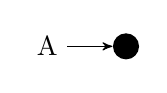
\begin{tikzpicture}[baseline=(A1), on grid]
        \node[] (A1) at (0, 0) {A};
        \node[circle,right of=A1, fill=black] (T) {};
        \draw[->] (A1) -- (T);
    \end{tikzpicture}
\end{equation}

\subsection{Forward control flow}

To account for control flow, we add a coproduct to our category, which we shall
denote by $\oplus$. Note that this is different from the $\otimes$ operation,
we have so far considered, and we are thus creating a \textbf{bimonoidal}
category, with two separate monoidal structures. Graphically, we will
indicate $\oplus$ by boxes around the operations in questions, so for example,
for the morphism $(f \oplus g) \otimes h: (A \oplus B) \otimes C \to (A^\prime \oplus B^\prime) \otimes C^\prime$,
we will draw:

\begin{equation}
    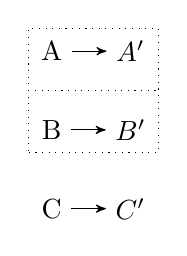
\begin{tikzpicture}[baseline=(B), on grid]
        \node[] (A) {A};
        \node[below of=A] (B) {B};
        \node[below of=B] (C) {C};

        \node[right of=A] (A') {$A^\prime$};
        \node[right of=B] (B') {$B^\prime$};
        \node[right of=C] (C') {$C^\prime$};

        \draw[->] (A) -- (A');
        \draw[->] (B) -- (B');
        \draw[->] (C) -- (C');

        \node[draw,dotted,fit=(A) (A') (B) (B'), inner sep = 1pt] (AA) {};
        \draw[dotted] (AA.west) -- (AA.east) {};
    \end{tikzpicture}
\end{equation}

Now, we have an operation $\varphi: A \oplus A \to A$, that joins control flow edges:

\begin{equation}
    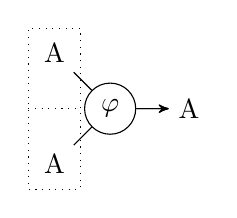
\begin{tikzpicture}[baseline=(A1), on grid]
        \node[] (A1) {A};
        \node[circle, draw, left of=A1] (C) {$\varphi$};
        \node[below left of=C] (A2) {A};
        \node[above left of=C] (A3) {A};

        \draw[->] (A2) -- (C) -- (A1);
        \draw[->] (A3) -- (C) -- (A1);
        \node[draw,dotted,fit=(A2)(A3), inner sep = 2pt] (AA) {};
        \draw[dotted] (AA.west) -- (AA.east) {};
    \end{tikzpicture}
\end{equation}

and we will introduce an additional "conditonal branch" operation $br: A \otimes C \to A \oplus A$ (where we say $C$
is the condition):

\begin{equation}
    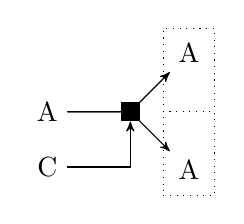
\begin{tikzpicture}[baseline=(A1), node distance = 3em and auto, on grid]
        \node[] (A1) at (0, 0) {A};
        \node[right of=A1, fill=black] (C) {};
        \node[node distance = 2em, below of=A1] (Cond) {C};
        \node[below right of=C] (A2) {A};
        \node[above right of=C] (A3) {A};
        \draw[->] (A1) -- (C.center) -- (A2);
        \draw[->] (A1) -- (C.center) -- (A3);
        \draw[->] (Cond) -| (C);
        \node[draw,dotted,fit=(A2)(A3), inner sep = 2pt] (AA) {};
        \draw[dotted] (AA.west) -- (AA.east) {};
    \end{tikzpicture}
\end{equation}

We further impose the following \textit{co-predication relation}:

\begin{equation}
    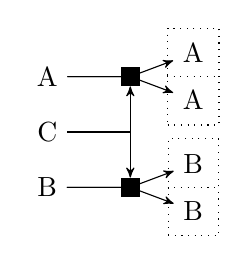
\begin{tikzpicture}[baseline=(Cond), node distance = 3em and auto, on grid]
        \node[] (A1) at (0, 0) {A};
        \node[right of=A1, fill=black] (CA) {};
        \node[node distance = 2em, below of=A1] (Cond) {C};
        \node[node distance = 2em, below of=Cond] (B1) {B};
        \node[right of=B1, fill=black] (CB) {};
        \node[above right=0.3 and 0.8 of CA] (A2) {A};
        \node[below right=0.3 and 0.8 of CA] (A3) {A};
        \node[below right=0.3 and 0.8 of CB] (B2) {B};
        \node[above right=0.3 and 0.8 of CB] (B3) {B};
        \draw[->] (A1) -- (CA.center) -- (A2);
        \draw[->] (A1) -- (CA.center) -- (A3);
        \draw[->] (Cond) -| (CA);
        \draw[->] (Cond) -| (CB);
        \draw[->] (B1) -- (CB.center) -- (B2);
        \draw[->] (B1) -- (CB.center) -- (B3);
        \node[draw,dotted,fit=(A2)(A3), inner sep = 2pt] (AA) {};
        \draw[dotted] (AA.west) -- (AA.east) {};
        \node[draw,dotted,fit=(B2)(B3), inner sep = 2pt] (BB) {};
        \draw[dotted] (BB.west) -- (BB.east) {};
    \end{tikzpicture} \hspace{1em}\cong
    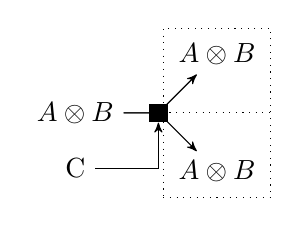
\begin{tikzpicture}[baseline=(A1), node distance = 3em and auto, on grid]
        \node[] (A1) at (0, 0) {$A\otimes B$};
        \node[right of=A1, fill=black] (C) {};
        \node[node distance = 2em, below of=A1] (Cond) {C};
        \node[below right of=C] (A2) {$A\otimes B$};
        \node[above right of=C] (A3) {$A\otimes B$};
        \draw[->] (A1) -- (C.center) -- (A2);
        \draw[->] (A1) -- (C.center) -- (A3);
        \draw[->] (Cond) -| (C);
        \node[draw,dotted,fit=(A2)(A3), inner sep = 2pt] (AA) {};
        \draw[dotted] (AA.west) -- (AA.east) {};
    \end{tikzpicture}
\end{equation}

As a notational convenience, we write $\oplus_c$ for the coproduct introduced
under some abstract condition $c$. In that case, we may write the co-predication
condition as
\[ \leftrightarrow_{\oplus} := (A \oplus_c B) \otimes (C \oplus_c D) \cong (A \otimes C) \oplus_c (B \otimes D) \]

To avoid running into technical difficulties, we further allow commuting arbitrary
morphisms through the branch operations, such that we can be sure every $A \oplus B$
is always potentially the direct result of a branch operation, such that we may
validly introduce abstract condition tags on any such $\oplus$ operation
\footnote{I realize this is a bit handwavy. While I believe this works fine, I would
be interested in improvements to make this construction more formal and
potentially avoid the reliance on commuting morphisms through the branch operation
so as ot facilitate the future addition of side effects.}.

\subsection{Lifting to the Optic category}

\subsubsection{Product Structure}

Having defined the structure for our bimonoidal category $SSA_{\mathcal{C}}$,
what can we say about the structure of $\text{Optic}_{SSA_{\mathcal{C}}}$?
To be explicit, we're still performing the optic construction with respect to
the $\otimes$ structure of our category. Let us first look at the product itself.
Do we have a diagonal map in $\text{Optic}_{SSA}$? Perhaps surprisingly, the answer
is no! To see this, let's consider what we must construct:

We wish to find a map $\text{Optic}(\Delta_{SSA}): (A, A') \to (A, A') \otimes (A, A')$.
A representative for such a morphism would have the form $\langle l, r \rangle$:
$l: A \to M \otimes A \otimes A$, $r: M \otimes A^\prime \otimes A^\prime \to A'$.
Finding $l$ is easy, we can just use $\Delta_{SSA}$ (letting $M=I$) from the underlying category.
However, there is no good way to construct $r$. A priori, there is no reason
to expect any morphism of the shape $A' \otimes A' \to A'$ to exist, and even
if such morphisms do exists, there is no reason to expect them to have the
required uniqueness properties. It is important to note that this does not
prevent us from lifting $\Delta_{SSA}$ to $\text{Optic}$ in our applications
of interest, it simply means that $\otimes$ is not a categorical product in
$\text{Optic}_{SSA_{\mathcal{C}}}$, so we must make make a choice of summation
morphism in our lifting functor.

\subsubsection{Coproduct Structure}

Given our utter disappointment with the product structure, can we have any
hope to lift the co-product structure. Yes, we do! First we construct the
co-product itself. For two optics $\langle l_1 | r_1 \rangle: (A, A') \to (B, B')$
with residual $M_1$ and $\langle l_2 | r_2 \rangle: (C, D') \to (D, D')$ with residual $M_2$,
we construct a new optic $\langle l_{12} | r_{12} \rangle$ where

\begin{equation}
\begin{split}
l_{12} = (l_1 \oplus l_2) \bbsemi \leftrightarrow_{oplus} \\
r_{12} = \leftrightarrow_{oplus}^{-1} \bbsemi (r_1 \oplus r_2)
\end{split}
\end{equation}

Similarly, we can confirm that this is indeed a coproduct by exhibting the $\varphi$
morphism. The trick here is to use the
residual to carry the branch history information. Perhaps the simplest
representative of $\text{Optic}(\varphi): (A \oplus_a A, A' \oplus_a A') \to (A, A')$ would be $\langle l | r \rangle$ where

\begin{equation}
\begin{split}
l &= \Delta_{SSA} \bbsemi (\text{id}_{A \oplus_a A} \otimes \varphi) \\
r &= d \bbsemi (\pi_2 \oplus \pi_2)
\end{split}
\end{equation}

where $d$ is the distributive map. While this may be a little abstract, hopefully
it becomes clear as a picture:

\begin{equation}
    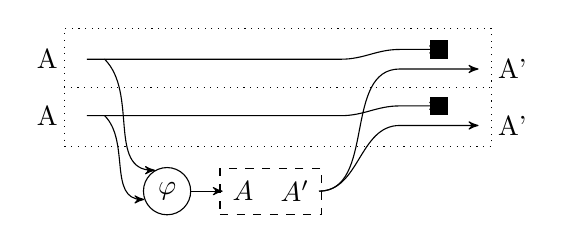
\begin{tikzpicture}[baseline=(S2)]
        \node (l) at (0, 0) {};

        \node (S1) [above left=0 and 0.2 of l.center,label=left:A,minimum height=2em] {};
        \node (S2) [below left=0 and 0.2 of l.center,label=left:A,minimum height=2em] {};
        \node (C1) [right=0.1 of S1] {};
        \node (C2) [right=0.1 of S2] {};

        \node (J1) [right=3.5 of C1] {};
        \node (J2) [right=3.5 of C2] {};

        \draw[->] (C1.center) to[out=east,in=west] ++(0.5,0.0) -- ++(2.5,0) to[out=east,in=west] (J1.north) -> ++(0.5,0) node[fill=black] {};
        \draw[->] (C2.center) to[out=east,in=west] ++(0.5,0.0) -- ++(2.5,0) to[out=east,in=west] (J2.north) -> ++(0.5,0) node[fill=black] {};
        \node[vert, below right=1.1 and 0.6 of C2] (phi) at (0, 0) {$\varphi$};

        \draw[->] (S1) -- (C1.center) to[out=south east,in=west] (phi.120);
        \draw[->] (S2) -- (C2.center) to[out=south east,in=west] (phi.200);

        \node (A) [right =0.4 of phi] {$A$};
        \node (A') [right =0.1 of A] {$A'$};

        \draw[->] (phi) -- (A);

        \draw[->] (A') to[out=east, in=west] (J1.south) -- ++(1,0) node[label=right:A'] (T1) {};
        \draw[->] (A') to[out=east, in=west] (J2.south) -- ++(1,0) node[label=right:A'] {};

        \node[draw,dashed,fit=(A) (A'), inner sep = 1pt] (AA) {};
        \node[draw,dotted,fit=(S1)(S2)(J1)(J2)(T1), inner sep = 1pt] (AA) {};
        \draw[dotted] (AA.west) -- (AA.east) {};

    \end{tikzpicture}
\end{equation}

Note that another representative of the same optic could simply record the
active component (e.g. by using the map $(x \to 1) \oplus (y \to 2)$ and
reintroducing a branch on the RHS).

However, note that (at least the way we chose to set it up) we do not have a
unique lifting of the branch operator itself.

\section{Optic Functors}

One useful way to construct optics is to do so automatically, from simpler
descriptions. More formally, we are interested in functors $F: \mathcal{C} \to \Optic_{\mathcal{D}}$.
The requirement for $F$ to be a functor means that composition in $\mathcal{C}$
matches composition in $\Optic_{\mathcal{D}}$, i.e. $F(f) \bbsemi F(g) = F(f \bbsemi g)$.
We shall call such functors (whose codomain is an optic category) \textit{optic functors}.

We have already seen an example of this kind of operation! In our definition
of \textit{FastSetIndex} above, we represented the optic, as a path of indices.
If we wanted to, we could consider this path of indices description a category
(e.g. the category in which objects are Julia datatypes and there is morphisms
from a datatype to each of its field types). In this case, the
optic functor is essentially the definitions of the \textit{left} and
\textit{right} generic, functions. Of course, we could have also left off the
subtype and instead defined a constructor of \textit{OpticRepr} with the
\textit{left} and \textit{right} definitions inline (such a constructor does
exist in our above definition, by virtue of the subtype). In that case, we
might want to check the functor law like so:

\begin{minted}[fontsize=\footnotesize,framesep=2mm]{julia}
julia> o₁ = OpticRepr(FastSetIndex(2) ⨟
                      FastSetIndex(1))
julia> o₂ = OpticRepr(FastSetIndex(2)) ⨟
            OpticRepr(FastSetIndex(1))
julia> o₁(c->c+100, tup)
(1, (102, 3))

julia> o₂(c->c+100, tup)
(1, (102, 3))
\end{minted}

However, it is import to emphasize that while optic functors are required to
preserve composition, when implemented as above, they are \textbf{not} required
to produce the same representative. Indeed, in our example:

\begin{minted}[fontsize=\footnotesize,framesep=2mm]{julia}
julia> o₁.l(tup)[1]
(1, (2, 3))

julia> o₂.l(tup)[1]
((1, (2, 3)), (2, 3))
\end{minted}

the two representatives $o_1$ and $o_2$ are not identical, even though they
represent the same optic.

\subsection{Optic functors on programs}

We now leave behind our trusty \textit{setindex} example and consider optic
functors from programs. To keep the discussion somewhat concrete, consider
the following example: Alice, Bob, and Clara are department heads at
Consolidated Widgets Incorporated. One day the anti-trust regulator decides that
Consolidated Widgets Inc is a little too consolidated and trisects the company
into AliceCo, BobCo and ClaraCo with the three former department heads promoted
to the CEOs of their respective companies. They now have a problem: While they
know how to manufacture widgets, they now also need to keep track of how much
each individual part costs and assign profits back to the appropriate company.
Can optic functors help? Yes!

Suppose the program for widget assembly is simply

\begin{center}
\begin{minted}[fontsize=\footnotesize,framesep=2mm]{julia}
widget(sweat, love) = C(A(sweat), B(love))
\end{minted}
\end{center}

i.e. Alice and Bob both manufacture subassemblies from raw inputes (sweat and love) and Clara handles
the final assembly). We wish to construct an optic functor $\textbf{\euro{}}$ that
takes in the widget construction function and spits out a function that both
constructs the widgets and accumulates prices on the left side of the optic,
and then distributes the profits on the right side of the optic after the widgets
have been sold. Now, we have four function of interest here $widget$, $A$, $B$
and $C$. For each of $A$, $B$ and $C$, we need to do some manual work.
Alice, Bob, and Clara need to do some manual work to figure out what their costs are.
We say that $A$, $B$ and $C$ are \textit{primitive} with respect to this functor.
Alright, let's suppose we have our prices (for simplicity $10\euro{}$ for Alice,
$20\euro{}$ for Bob and $30\euro{}$ for Clara). We will also give each of them
a flat $30\%$ profit margin. We will use the continuation
encoding of the optic to specify the value of $\textbf{\euro{}}$ on each of our
primitives:

\begin{snippet}
|$\textbf{\euro{}}$|A(price, sweat) = let cost=|$10$|;
  (price + cost, A(sweat)),
    profit->(profit - cost * 1.3)
end
|$\textbf{\euro{}}$|B(price, love) = let cost=|$20$|;
  (price + cost, B(love)),
    profit->(profit - cost * 1.3)
end
\end{snippet}

$C$ is a little more tricky. For $C$, we have two arguments, so on right side
of the optic, we need to produce two outputs. There are several ways to model
this. We could consider only allowing function with a single input and a single
output, together with primitive operations for packing (into a tuple) and
unpacking, or we could simply require the output to always be a tuple whose
length matches the original number of arguments. Here we pick the latter
encoding and write:

\begin{snippet}
|$\textbf{\euro{}}$|C(aprice, bprice, a, b) = let cost=|$30$|;
  (aprice + bprice + cost, C(a, b)),
    profit->(take(profit, aprice),
             take(profit, bprice))
end
\end{snippet}

Ok, phew that was a bit of work to figure out all the primitives. However, now
that this is done, we do get some reward for our efforts. We get the definition
of $\textbf{\euro{}}widget$ for free by applying the functor law. Recall that
we essentially defined $widget = (A \otimes B) \bbsemi C$. Thus, applying the
functor law, we immediately get that $\textbf{\euro{}}widget = (\textbf{\euro{}}A \otimes \textbf{\euro{}}B) \bbsemi \textbf{\euro{}}C$

By tracing through definitions, we can write out an explicit representative in
the continuation encoding:

\begin{snippet}
function |\textbf{\euro{}}|widget(sweat_cost, love_cost, sweat, love)
  aprice, |$a$|, |$a^\star$| = |\textbf{\euro{}}A|(sweat_cost, sweat)
  bprice, |$b$|, |$b^\star$| = |\textbf{\euro{}}B|(love_cost, love)
  price, |$c$|, |$c^\star$| = |\textbf{\euro{}}C|(aprice, bprice, a, b)
  price, |$c$|, profit->begin
    (|$a^\dagger$|,|$b^\dagger$|) = |$c^\star$|(profit)
    |$\text{love}^\dagger$| = |$b^\star$|(|$b^\dagger$|)
    |$\text{sweat}^\dagger$| = |$a^\star$|(|$a^\dagger$|)
    (|$\text{sweat}^\dagger$|, |$\text{love}^\dagger$|)
  end
end
\end{snippet}

Now, this might seem a bit complicated (and it is), but that is precisely the
point. Writing this out explicitly is quite tedious, but there are no choices
to be made in how it is written. \textbf{Once we have defined the optic functor on the
requisite primitives, we can make use of the composition law to generate a
representative of the functor applied to any function that is a composition
for our primitives.}

\subsection{Some notation}

As we saw in the previous section, the explicit representatives generated by
optic functors can be quite complicated. To avoid getting lost, we should make
some notational conventions. To begin with, we shall consider input programs
to be represented by their SSA form representation. We shall assume that the
reader is familiar with SSA form IR (if not, see the Julia devdocs on SSA form
IR). Now, let $\textbf{\euro{}}$ be an optic functor. In the context of applying
$\textbf{\euro{}}$ to some function $f$, we shall say that $f$ is the \textit{primal
function} and similarly we shall call the value computed by $f$ the \textit{primal value}.
From now on, we will generally be working with the continuation
encoding of an optic. By abuse of notation, we will write $\textbf{\euro{}} f$
for the function that is the canonical representative of the optic in
continuation encoding (canonical here meaning obtained by straightforward
application of the functor laws). We shall call this function the \textit{optic
 function}. We shall call the value returned from the optic function the \textit{focal bundle}.
Since we sometimes want to look at it in isolation, we will call
the continuation generated by the optic function, the \textit{pullback function},
written $f^\star$ for some primal function $f$. Since $f^\star$ depends on the
representative, unless otherwise specified, $f^\star$ shall refer to the pullback
function generated by the canonical optic function.

When looking at SSA form, IR, for some SSA value $\%a = A(...)$ in the primal function,
we will write $(\%a, \%a^\star) = \textbf{\euro{}} A(...)$ in the optic function.
The intended implication here is that $\%a$ in the optic function is the same value
as $\%a$ in the primal function. This will generally be the case, as long as
the optic primitives obey this constraint. However, we have not required this
invariant on primitives in our definition of the optic functor and there are
(rare) cases in which it is useful for these to be different. Where the
distinction matters, the context should be explicitly specified.
Lastly, we look at the pullback function. By the optic composition law,
pullbacks behave contravariantly to the primal function, so for a call
$c = C(A, B)$ in the primal function, we will have a call
$(\%a^\dagger, \%b^\dagger) = \underline{\%c^\star}(\%c^\dagger)$. Where in general
an underline indicates that a value was captured from the optic function.

\subsection{Optic functors from SSA IR}

When we discussed SSA form in section \ref{ssair}, we identified several
structural features of the IR that did not lift uniquely to the optic category.
In particular, this means that we have some freedom in choosing how these should
lift for our optic functor. In particular, the structural aspects of SSA IR that
did not have a unique lift were:

\begin{itemize}
\item Copy
\item Delete
\item Conditional Branch
\end{itemize}

As an exercise, let us go through these and choose an implementation.

\subsubsection{Copy}

In our little widget manufacturing example from the previous section, the objects
being propagated in the primal functions were in general intermediate products
that could only be used. But what happens if we introduce trivially copyable
goods into the equation? E.g. suppose Alice and Bob both gain a trivially
copyable input (perhaps music they like to listen to, or maybe they both
require a license for JuliaPro), and that Dave produces such an input.
For simplicity, we will also drop Alice and Bob's other inputs. We have a new
program:

\begin{snippet}
function clonewidget()
    d = D()
    a = A(d)
    b = B(d)
    c = C(a, b)
end
\end{snippet}

Let us look at some sensible policy choices\footnote{Welcome to Copyright 101 - Today's topic: Category theory.} we might make.
For example, we could decide that David gets to decide what to charge for each copy of `d':

\begin{snippet}
function |$\textbf{\euro{}}$|clone(dprice, d)
    (dprice, dprice), (d, d),
    (profit₁, profit₂)->(profit₁ + profit₂)
end
\end{snippet}

or maybe everybody pays a fixed fee, independent of David's costs:

\begin{snippet}
function |$\textbf{\euro{}}$|clone(dprice, d)
    (1, 1), (d, d),
    (profit₁, profit₂)->(profit₁ + profit₂)
end
\end{snippet}

or maybe everybody pirates his music and David gets payed nothing:

\begin{snippet}
function |$\textbf{\euro{}}$|clone(dprice, d)
    (0, 0), (d, d),
    (profit₁, profit₂)->0
end
\end{snippet}

or maybe the participants of our economy are playing hot potato, and always
exactly one of the participants needs to pay:

\begin{snippet}
function |$\textbf{\euro{}}$|clone(dprice, d)
    rand(Bool) ? (dprice, 0) : (0, dprice), (d, d),
    (profit₁, profit₂)->(profit₁ + profit₂)
end
\end{snippet}

However, note that while this is a valid definition under our definition of
an optic functor, applying $textbf{\euro{}}$ now leads to accumulation order
dependence (the same happens in the variant where cloning is done once per value).
As a result, $textbf{\euro{}}$ would no longer preserve standard SSA invariants.
This is legal according to our definition, but it can be convenient to be able to
arbitrarily permute SSA transforms and optic functors. Thus, we would generally
only ever choose one of the first two definitions.

\subsubsection{Delete}

Like copy, we have some freedom what do here. For our example, it would probably
make sense to dynamically disallow deleting objects that have a non-zero price,
so we might write:

\begin{snippet}
function |$\textbf{\euro{}}$|delete(dprice, d)
    dprice != 0 && error("Who's gonna pay for that?")
    ()->(0,)
end
\end{snippet}

\subsubsection{Branch}

Again we have several potential choices. The primary reason that the branch
operation was non-canonical was because of the implicit delete of the branch
condition. However, it is possible for us to implement more complicated
behaviors. For example suppose we wanted to proportionately assign to each
input. We might write something like (encoding for the branch functor is
slightly tricky, this is one example):

\begin{snippet}
function |$\textbf{\euro{}}$|branch(aprices, cprice, as, c)
    # Smear the cost of `c' proportionately
    total_a = sum(aprices)
    aprices = map(p->p*(1 + cprice/total_a), aprices)
    aprices, (c, as), profit->begin
        (profit - cprice), cprice
    end
end
\end{snippet}

However, as with the prior discussion, this would not match standard ssa behavior
(i.e. programs equivalent under SSA would not longer be equivalent when lifted).
As before, this is legal, but may not be desirable.

\section{Tangent spaces}

We will briefly define the concepts relevant to us, but otherwise defer to any
introductory text on differential geometry \footnote{e.g. https://faculty.math.illinois.edu/~lerman/518/f11/8-19-11.pdf}. Let $M$ be a smooth manifold,
$C^\infty(M)$ the space of smooth functions on $M$. A tangent vector $\nu$ to $M$
at $a$ is an $\mathbb{R}$-linear derivation from $C^\infty(M)$ into $\mathbb{R}$,
i.e. a function from $C^\infty(M) \to \mathbb{R}$ satisfying:

\begin{equation}
\nu(f \cdot g)(x) = g(a)\cdot \nu(f) + f(a) \cdot \nu(g)
\end{equation}

The collection of all tangent vectors to $M$ at $a$ form a vector space, called
the tangent space to $M$ at $a$, $T_a M$. Additionally, if we glue all these
vector spaces together, we obtain the tangent bundle $T M$.

We can dualize this vector space and obtain the cotangent bundle $T^\star M$.
Sections of the cotangent bundle are also called differential 1-forms.

If we have a function between manifolds, say $f: M \to N$, we obtain a pushforward
of tangent spaces: $f_\star: T_M \to T_N$ given by:

\begin{equation}
(f_\star \nu) g = \nu(g \circ f)
\end{equation}

(for $g: C^\infty(M)$), as well as a pullback of cotangent spaces $f^\star: T^\star N \to T^\star M$
given by

\begin{equation}
(f^\star dx) \nu = dx(f_\star \nu)
\end{equation}

These notions are generalizations of some of the standard notions of derivatives
that may be familiar from multivariable calculus. Suppose $f: \R^n \to \R^m$,
Let $\pi_i$ be the component projection function. We obtain a canonical basis,
of the tangent space $T \R^n$ given by the unique functions such that
\begin{equation}
\nu_i (\pi_j) = i == j
\end{equation}
And similarly for the cotangent space.

Now the Jacobian $J f$ defined by

\begin{equation}
(J f)_{ij} = \frac{\partial f_i}{\partial x_j}
\end{equation}

is just matrix obtained by pushing forward the standard basis fo $T \R^n$ using
$f_\star$. Equivalently, it is the transpose of the pullback of the standard
basis of $T^\star \R^m$.

As a special case suppose $m=1$. Then we have a function $\nabla f: \R^n \to \R$,
the gradient of $f$ at $x$. Using our language, this is simply the pullback of
the differential one form $dx_1$ from $T^* \R$.

\section{Advanced Optics considerations}

\subsection{Action of an Optic on the underlying category}

The category $\Optic_\mathcal{C}$ acts on the underlying category $\mathcal{C}$
in the following sense: We have a contravariant functor $p: \Optic_\mathcal{C} \to \text{Set}$
that assigns to every object $(A, A^\prime)$ the set $Hom(A, A\prime)$ and to
morphisms $\langle l | r \rangle$ the morphism $p \langle l | r \rangle: Hom(B, B\prime) \to Hom(A, A\prime)$
given by:
\[
p \langle l | r \rangle f = l \bbsemi (id_M \otimes f) \bbsemi r
\]

or graphically by assigning to a morphism $f \in \Hom(B, B^\prime)$ the morphism
obtained by plugging $f$ into the "hole" of the optic:

\begin{equation}
    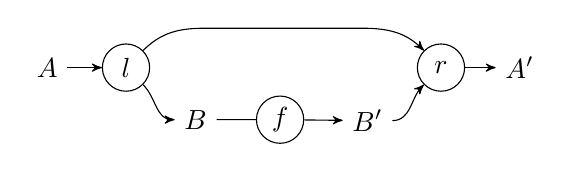
\begin{tikzpicture}[baseline=(S)]
        \node[vert] (l) at (0, 0) {$l$};
        \node[vert] (r) at (4, 0) {$r$};

        \node (S) [left of=l] {$A$};
        \node (A) [below right = 0.2 and 0.4 of l] {$B$};
        \node (S') [right of=r] {$A'$};
        \node (A') [below left = 0.2 and 0.4 of r] {$B'$};

        \node[vert, right=0.5 of A] (f) {$f$};

        \draw[->] (S) -- (l);
        \draw[->] (l) to[out=south east,in=west] (A);

        \draw[<-] (S') -- (r);
        \draw[<-] (r) to[out=south west,in=east] (A');

        \draw[->] (l) to[out=north east, in=west] ++(1,0.5)
         to ++(2,0)
         to[out=east, in=north west] (r)
        ;

        \draw[->] (A) -- (f) -- (A');
    \end{tikzpicture}
\end{equation}


\subsection{Higher order optics}

As hinted at above and proven in detail in Riley \cite{riley:optics}, $\Optic$
is an endofunctor on the category of symmetric monoidal categories, i.e. for
a symmetric monoidal category $\mathcal{C}$, $\Optic_{\mathcal{C}}$ is once again
a symmetric monoidal category. In particular, this means we may repeat the
application of $\Optic$ to obtain higher order optics. Let us explicitly
characterize second order optics such that we may discuss some features that
will come in later. Objects in $\Optic_{\Optic_{\mathcal{C}}}$ are pairs of
objects in $\Optic_{\mathcal{C}}$, i.e. in general quadruplets of objects in
the original category. We will write $\left(\begin{array}{cc} (A_1 & A_2) \\ (A_3 & A_4) \end{array}\right)$
for the higher order optic that pairs the objects $\left(\begin{array}{cc} A_1 \\ A_2\end{array}\right)$
$\left(\begin{array}{cc} A_3 \\ A_4\end{array}\right)$ from the original optic category.
Then a representative of the optic morphisms
$\Optic\left(\left(\begin{array}{cc} (A_1 & A_2) \\ (A_3 & A_4) \end{array}\right),
\left(\begin{array}{cc} (B_1 & B_2) \\ (B_3 & B_4) \end{array}\right)\right)$,
is a pair of optics $\langle \mathcal{O}_l | \mathcal{O}_r \rangle$ where
\begin{equation}
\begin{split}
\mathcal{O}_l \in \Optic\left(\left( \begin{array}{c} A_1 \\ A_2 \end{array} \right),
\left( \begin{array}{c} M_\mathcal{O} \\ M_\mathcal{O}^\prime \end{array} \right) \otimes
\left( \begin{array}{c} B_1 \\ B_2 \end{array} \right)
\right)
\\
\mathcal{O}_r \in \Optic\left(
\left( \begin{array}{c} M_\mathcal{O} \\ M_\mathcal{O}^\prime \end{array} \right) \otimes
\left( \begin{array}{c} B_3 \\ B_4 \end{array} \right),
\left( \begin{array}{c} A_4 \\ A_4 \end{array} \right)
\right)
\end{split}
\end{equation}

. We take representatives $\langle l_l | r_l \rangle$ of $\mathcal{O}_l$
and $\langle l_r | r_r \rangle$ of $\mathcal{O}_r$ with residuals $M_l$ and $M_r$
respectively. Writing the morphisms out algebraically is a bit confusing, so
let's look at the graphical representation:

\begin{equation}
    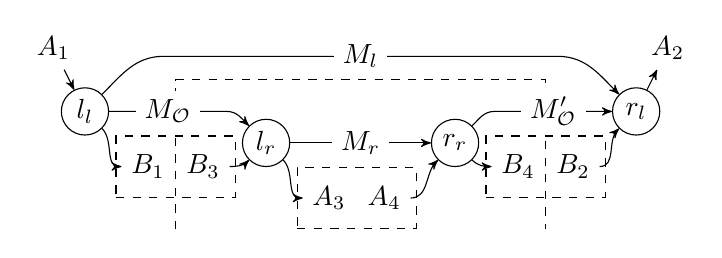
\begin{tikzpicture}[on grid, baseline=(ll)]
        \node[vert] (ll) at (0, 0) {$l_l$};
        \node[vert, right=2.3 of ll, yshift=-4mm] (lr) {$l_r$};
        \node[vert, right=7 of ll] (rr) {$r_l$};
        \node[vert, left=2.3 of rr, yshift=-4mm] (rl) {$r_r$};

        \node (A1) [above left=0.8 and 0.4 of ll] {$A_1$};
        \node (A2) [above right=0.8 and 0.4 of rr] {$A_2$};

        \node (B1) [below right=0.7 and 0.8 of ll] {$B_1$};
        \node (B3) [right=0.7 of B1] {$B_3$};

        \node (A3) [below right=0.7 and 0.8 of lr] {$A_3$};
        \node (A4) [right=0.7 of A3] {$A_4$};

        \node (B2) [below left=0.7 and 0.8 of rr] {$B_2$};
        \node (B4) [left=0.7 of B2] {$B_4$};

        \node[draw,dashed,fit=(B1) (B3), inner xsep = 2pt] (box1) {};
        \node[draw,dashed,fit=(A3) (A4), inner xsep = 2pt] (box2) {};
        \node[draw,dashed,fit=(B2) (B4), inner xsep = 2pt] (box3) {};
        \draw[dashed] ($(box1.south) - (0,0.4)$) -- ++(0,1.9) -- ($(box3.south) + (0,1.5)$) -- ($(box3.south) - (0,0.4)$);

        \draw [->] (A1) -- (ll);
        \draw [->] (rr) -- (A2);

        \draw [->] (ll) -- ++(1.8,0) node[midway, fill=white] {$M_{\mathcal{O}}$} to[out=east, in=north west] (lr);
        \draw [->] (ll) to[out=south east,in=west] (B1);
        \draw [->] (B3) to[out=east,in=south west] (lr);

        \draw [->] (lr) -- node[midway, fill=white] {$M_r$} (rl);
        \draw [->] (lr) to[out=south east,in=west] (A3);
        \draw [->] (A4) to[out=east,in=south west] (rl);

        \draw [->] (rl) to[out=north east, in=west] ($(rr)-(1.8,0)$) -- node[midway, fill=white] {$M_{\mathcal{O}}^\prime$} (rr);
        \draw [->] (rl) to[out=south east,in=west] (B4);
        \draw [->] (B2) to[out=east,in=south west] (rr);

        \draw[->] (ll) to[out=north east, in=west] ++(1,0.7)
         -- ++(5,0) node[midway,fill=white] {$M_l$}
         to[out=east, in=north west] (rr)
        ;
    \end{tikzpicture}
\end{equation}

Here the dashed line plays the same role it did in the original diagram of
the optic: To compose optics, we "slice" along the dashed line and insert
the next higher order optic in the middle. To illustrate the composition,
we will first look at two diagrams stacked on top of each other using the
same structure as in the previous diagram, to make the flow of operations
obvious.

\begin{equation}
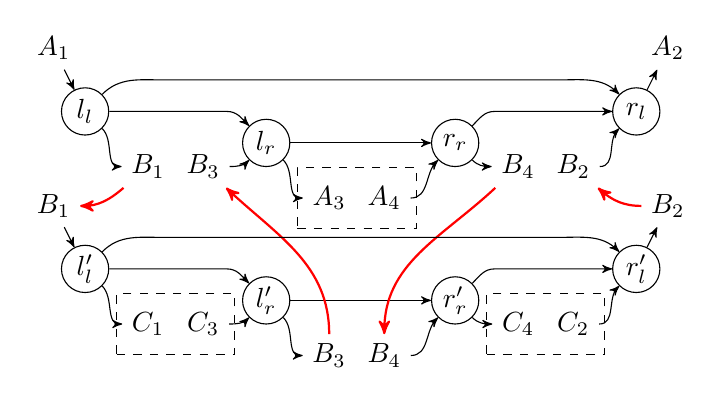
\begin{tikzpicture}[on grid]
    \node[vert] (ll) at (0, 0) {$l_l$};
    \node[vert, right=2.3 of ll, yshift=-4mm] (lr) {$l_r$};
    \node[vert, right=7 of ll] (rr) {$r_l$};
    \node[vert, left=2.3 of rr, yshift=-4mm] (rl) {$r_r$};

    \node (A1) [above left=0.8 and 0.4 of ll] {$A_1$};
    \node (A2) [above right=0.8 and 0.4 of rr] {$A_2$};

    \node (B1) [below right=0.7 and 0.8 of ll] {$B_1$};
    \node (B3) [right=0.7 of B1] {$B_3$};

    \node (A3) [below right=0.7 and 0.8 of lr] {$A_3$};
    \node (A4) [right=0.7 of A3] {$A_4$};

    \node (B2) [below left=0.7 and 0.8 of rr] {$B_2$};
    \node (B4) [left=0.7 of B2] {$B_4$};

    \draw [->] (A1) -- (ll);
    \draw [->] (rr) -- (A2);

    \draw [->] (ll) -- ++(1.8,0) to[out=east, in=north west] (lr);
    \draw [->] (ll) to[out=south east,in=west] (B1);
    \draw [->] (B3) to[out=east,in=south west] (lr);

    \draw [->] (lr) -- (rl);
    \draw [->] (lr) to[out=south east,in=west] (A3);
    \draw [->] (A4) to[out=east,in=south west] (rl);

    \draw [->] (rl) to[out=north east, in=west] ($(rr)-(1.8,0)$) -- (rr);
    \draw [->] (rl) to[out=south east,in=west] (B4);
    \draw [->] (B2) to[out=east,in=south west] (rr);

    \draw[->] (ll) to[out=north east, in=west] ++(1,0.4)
     to ++(5,0)
     to[out=east, in=north west] (rr)
    ;

    \node[draw,dashed,fit=(A3) (A4), inner xsep = 2pt] (box2) {};

    \node[vert, below=2 of ll] (ll_2) {$l_l^\prime$};
    \node[vert, right=2.3 of ll_2, yshift=-4mm] (lr_2) {$l_r^\prime$};
    \node[vert, right=7 of ll_2] (rr_2) {$r_l^\prime$};
    \node[vert, left=2.3 of rr_2, yshift=-4mm] (rl_2) {$r_r^\prime$};

    \node (B1_2) [above left=0.8 and 0.4 of ll_2] {$B_1$};
    \node (B2_2) [above right=0.8 and 0.4 of rr_2] {$B_2$};

    \node (C1) [below right=0.7 and 0.8 of ll_2] {$C_1$};
    \node (C3) [right=0.7 of C1] {$C_3$};

    \node (B3_2) [below right=0.7 and 0.8 of lr_2] {$B_3$};
    \node (B4_2) [right=0.7 of B3_2] {$B_4$};

    \node (C2) [below left=0.7 and 0.8 of rr_2] {$C_2$};
    \node (C4) [left=0.7 of C2] {$C_4$};

    \draw [->] (B1_2) -- (ll_2);
    \draw [->] (rr_2) -- (B2_2);

    \draw [->] (ll_2) -- ++(1.8,0) to[out=east, in=north west] (lr_2);
    \draw [->] (ll_2) to[out=south east,in=west] (C1);
    \draw [->] (C3) to[out=east,in=south west] (lr_2);

    \draw [->] (lr_2) -- (rl_2);
    \draw [->] (lr_2) to[out=south east,in=west] (B3_2);
    \draw [->] (B4_2) to[out=east,in=south west] (rl_2);

    \draw [->] (rl_2) to[out=north east, in=west] ($(rr_2)-(1.8,0)$) -- (rr_2);
    \draw [->] (rl_2) to[out=south east,in=west] (C4);
    \draw [->] (C2) to[out=east,in=south west] (rr_2);

    \draw [->,thick,color=red] (B1)  to[out=south west, in=east] (B1_2);
    \draw [->,thick,color=red] (B3_2) to[out=north, in=south east] (B3);
    \draw [->,thick,color=red] (B4) to[out=south west, in=north] (B4_2);
    \draw [->,thick,color=red] (B2_2) to[out=west, in=south east] (B2);

    \node[draw,dashed,fit=(C1) (C3), inner xsep = 2pt] (box1) {};
    \node[draw,dashed,fit=(C2) (C4), inner xsep = 2pt] (box3) {};

    \draw[->] (ll_2) to[out=north east, in=west] ++(1,0.4)
     to ++(5,0)
     to[out=east, in=north west] (rr_2)
    ;
\end{tikzpicture}

\end{equation}

We can relayout this to make the four segments more obvious. This is done in
figure \ref{2comphor}. Now, if $\euro{}: \mathcal{C} \to \Optic_\mathcal{C}$ is an
optic functor, then since it is monoidal functor, it immediately lifts to a functor:
$\euro: \Optic_{\mathcal{C}} \to \Optic_{\Optic_\mathcal{C}}$. Note that optics
constructed in this way will generally be more constrained than the full optics
construction. For example, the 2-optic we constructed above has objects that
are in general $4$-tuples $((A_1, A_2), (A_3, A_4))$ and more generally an $n$-optic
will have objects are $2^n$ tuples of objects in the base category. However,
if we obtain an optic by repeated application of an optic functor, several
of these objects will be the same and we will generally have $1+n$ different
objects of the base category in play. E.g. $\euro \euro f$ for some
morphism $f: A\to B$, would give a 2-optic $((A, A'),(A', A'')) \to ((B,B'),(B',B''))$.

For completeness, let us repeat this diagram, making use of the notation we established
above for optic obtained from optic functors:


\begin{equation}
    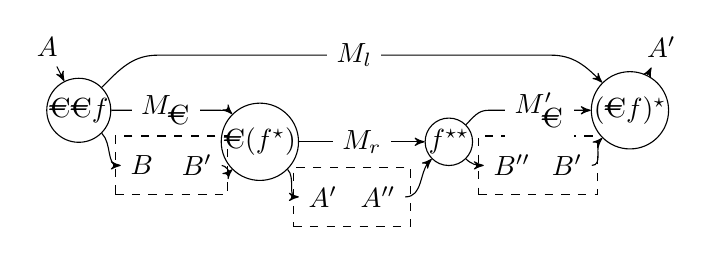
\begin{tikzpicture}[on grid]
        \node[vert] (ll) at (0, 0) {$\euro \euro f$};
        \node[vert, right=2.3 of ll, yshift=-4mm] (lr) {$\euro(f^\star)$};
        \node[vert, right=7 of ll] (rr) {$(\euro f)^\star$};
        \node[vert, left=2.3 of rr, yshift=-4mm] (rl) {$f^{\star\star}$};

        \node (A1) [above left=0.8 and 0.4 of ll] {$A$};
        \node (A2) [above right=0.8 and 0.4 of rr] {$A'$};

        \node (B1) [below right=0.7 and 0.8 of ll] {$B$};
        \node (B3) [right=0.7 of B1] {$B'$};

        \node (A3) [below right=0.7 and 0.8 of lr] {$A'$};
        \node (A4) [right=0.7 of A3] {$A''$};

        \node (B2) [below left=0.7 and 0.8 of rr] {$B'$};
        \node (B4) [left=0.7 of B2] {$B''$};

        \node[draw,dashed,fit=(B1) (B3), inner xsep = 2pt] (box1) {};
        \node[draw,dashed,fit=(A3) (A4), inner xsep = 2pt] (box2) {};
        \node[draw,dashed,fit=(B2) (B4), inner xsep = 2pt] (box3) {};

        \draw [->] (A1) -- (ll);
        \draw [->] (rr) -- (A2);

        \draw [->] (ll) -- ++(1.8,0) node[midway, fill=white] {$M_{\euro}$} to[out=east, in=north west] (lr);
        \draw [->] (ll) to[out=south east,in=west] (B1);
        \draw [->] (B3) to[out=east,in=south west] (lr);

        \draw [->] (lr) -- node[midway, fill=white] {$M_r$} (rl);
        \draw [->] (lr) to[out=south east,in=west] (A3);
        \draw [->] (A4) to[out=east,in=south west] (rl);

        \draw [->] (rl) to[out=north east, in=west] ($(rr)-(1.8,0)$) -- node[midway, fill=white] {$M_{\euro}^\prime$} (rr);
        \draw [->] (rl) to[out=south east,in=west] (B4);
        \draw [->] (B2) to[out=east,in=south west] (rr);

        \draw[->] (ll) to[out=north east, in=west] ++(1,0.7)
         -- ++(5,0) node[midway,fill=white] {$M_l$}
         to[out=east, in=north west] (rr)
        ;
    \end{tikzpicture}
\end{equation}

\begin{figure*}
    \begin{center}
    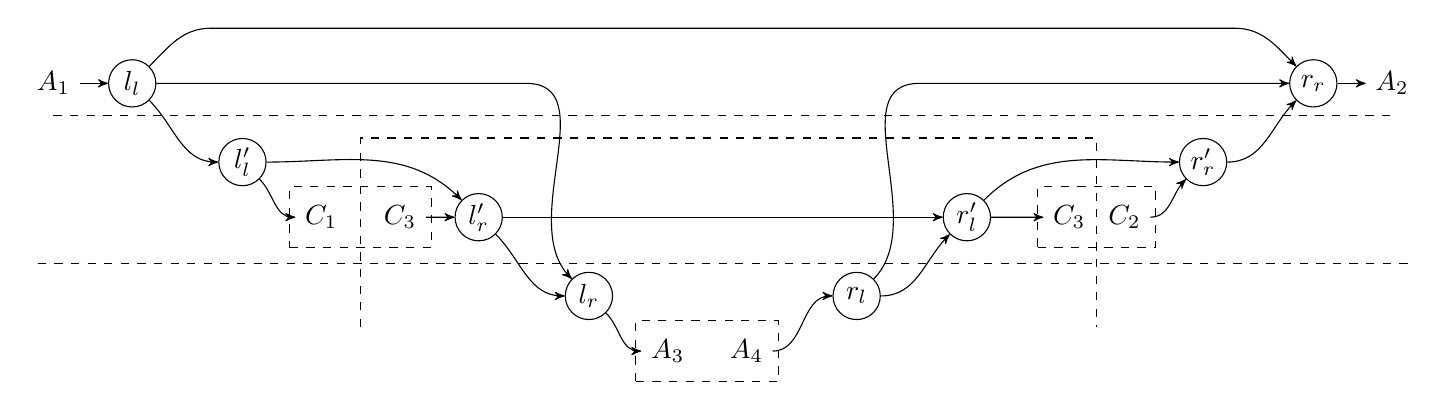
\begin{tikzpicture}[on grid]

        \node[vert] (ll) at (0, 0) {$l_l$};
        \node[vert, right=1.4 of ll, yshift=-10mm] (ll') {$l_l^\prime$};
        \node[vert, right=3 of ll', yshift=-7mm] (lr') {$l_r^\prime$};
        \node[vert, right=1.4 of lr', yshift=-10mm] (lr) {$l_r$};

        \node[vert, right=15 of ll] (rr) {$r_r$};
        \node[vert, left=1.4 of rr, yshift=-10mm] (rr') {$r_r^\prime$};
        \node[vert, left=3 of rr', yshift=-7mm] (rl') {$r_l^\prime$};
        \node[vert, left=1.4 of rl', yshift=-10mm] (rl) {$r_l$};

        \node[left=of ll] (A1) {$A_1$};
        \node[right=of rr] (A2) {$A_2$};

        \node (C1) [below right=0.7 and 1 of ll'] {$C_1$};
        \node (C3) [right=of C1] {$C_3$};

        \node (C2) [below left=0.7 and 1 of rr'] {$C_2$};
        \node (C4) [left=0.7 of C2] {$C_3$};

        \node (A3) [below right=0.7 and 1 of lr] {$A_3$};
        \node (A4) [right=of A3] {$A_4$};


        \draw[->] (ll) to[out=north east, in=west] ++(1,0.7)
         to ++(13,0)
         to[out=east, in=north west] (rr)
        ;

        \draw [->] (ll) -- ++(5,0) to[out=east, in=north west] (lr);
        \draw [->] (ll) to[out=south east, in=west] (ll');

        \draw [->] (ll') to[out=south east, in=west] (C1);
        \draw [->] (C3) to[out=east, in=west] (lr');
        \draw [->] (ll') to[out=east, in=north west] (lr');

        \draw [->] (lr') -- (rl');
        \draw [->] (lr') to[out=south east, in=west] (lr);

        \draw [->] (lr) to[out=south east, in=west] (A3);
        \draw [->] (A4) to[out=east, in=west] (rl);

        \draw [->] (rl) to[out=east, in=south west] (rl');

        \draw [->] (rl') to[out=north east, in=west] (rr');
        \draw [->] (rr') to[out=east, in=south west] (rr);

        \draw [->] (rl') -- (C4);
        \draw [->] (C2) to[out=east,in=south west] (rr');

        \draw [->] (rl) to[out=north east, in=west] ($(rr) - (5,0)$) -- (rr);

        \draw [->] (A1) -- (ll);
        \draw [->] (rr) -- (A2);

        \node[draw,dashed,fit=(C1) (C3), inner xsep = 2pt] (box1) {};
        \node[draw,dashed,fit=(A3) (A4), inner xsep = 2pt] (box2) {};
        \node[draw,dashed,fit=(C2) (C4), inner xsep = 2pt] (box3) {};

        \draw[dashed] ($(box1.south) - (0,1)$) -- ($(box1.south) + (0,1.4)$) -- ($(box3.south) + (0,1.4)$) -- ($(box3.south) - (0,1)$);

        \draw[dashed] ($(ll.south) - (1,0.1)$) -- ($(rr.south) + (1,-0.1)$);
        \draw[dashed] ($(lr.north) - (7,-0.1)$) -- ($(rl.north) + (7,0.1)$);
    \end{tikzpicture}
    \end{center}
    \caption{Composition of two second order optics layed out horizontally. Indicated by dashed lines are the cut/glue lines
    of the original optic (as well as the resulting optic, which corresponds with the cutline of the second optic).}
    \label{2comphor}
\end{figure*}

For completeness, let us proceed for one more step and explicitly draw a 3-optic.
As before, we have a pair of two 2-optics:


\begin{equation}
    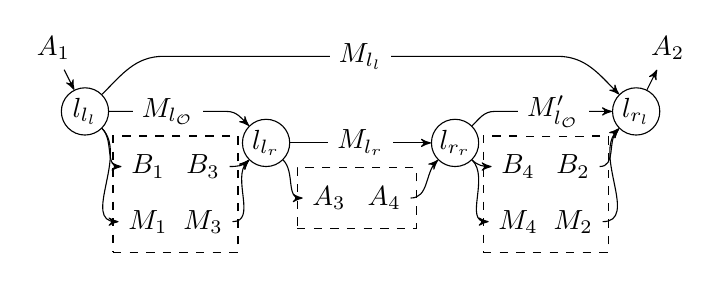
\begin{tikzpicture}[on grid]
        \node[vert] (ll) at (0, 0) {$l_{l_l}$};
        \node[vert, right=2.3 of ll, yshift=-4mm] (lr) {$l_{l_r}$};
        \node[vert, right=7 of ll] (rr) {$l_{r_l}$};
        \node[vert, left=2.3 of rr, yshift=-4mm] (rl) {$l_{r_r}$};

        \node (A1) [above left=0.8 and 0.4 of ll] {$A_1$};
        \node (A2) [above right=0.8 and 0.4 of rr] {$A_2$};

        \node (B1) [below right=0.7 and 0.8 of ll] {$B_1$};
        \node (B3) [right=0.7 of B1] {$B_3$};

        \node (M1) [below=0.7 of B1] {$M_1$};
        \node (M3) [below=0.7 of B3] {$M_3$};

        \node (A3) [below right=0.7 and 0.8 of lr] {$A_3$};
        \node (A4) [right=0.7 of A3] {$A_4$};

        \node (B2) [below left=0.7 and 0.8 of rr] {$B_2$};
        \node (B4) [left=0.7 of B2] {$B_4$};

        \node (M2) [below=0.7 of B2] {$M_2$};
        \node (M4) [below=0.7 of B4] {$M_4$};

        \node[draw,dashed,fit=(B1) (B3) (M1) (M3), inner xsep = 2pt] (box1) {};
        \node[draw,dashed,fit=(A3) (A4), inner xsep = 2pt] (box2) {};
        \node[draw,dashed,fit=(B2) (B4) (M2) (M4), inner xsep = 2pt] (box3) {};

        \draw [->] (A1) -- (ll);
        \draw [->] (rr) -- (A2);

        \draw [->] (ll) -- ++(1.8,0) node[midway, fill=white] {$M_{l_{\mathcal{O}}}$} to[out=east, in=north west] (lr);
        \draw [->] (ll) to[out=south east,in=west] (B1);
        \draw [->] (ll) to[out=south east,in=west] (M1);
        \draw [->] (B3) to[out=east,in=south west] (lr);
        \draw [->] (M3) to[out=east,in=south west] (lr);

        \draw [->] (lr) -- node[midway, fill=white] {$M_{l_r}$} (rl);
        \draw [->] (lr) to[out=south east,in=west] (A3);
        \draw [->] (A4) to[out=east,in=south west] (rl);

        \draw [->] (rl) to[out=north east, in=west] ($(rr)-(1.8,0)$) -- node[midway, fill=white] {$M_{l_\mathcal{O}}^\prime$} (rr);
        \draw [->] (rl) to[out=south east,in=west] (B4);
        \draw [->] (rl) to[out=south east,in=west] (M4);
        \draw [->] (B2) to[out=east,in=south west] (rr);
        \draw [->] (M2) to[out=east,in=south west] (rr);

        \draw[->] (ll) to[out=north east, in=west] ++(1,0.7)
         -- ++(5,0) node[midway,fill=white] {$M_{l_l}$}
         to[out=east, in=north west] (rr)
        ;
    \end{tikzpicture}
\end{equation}

\begin{equation}
    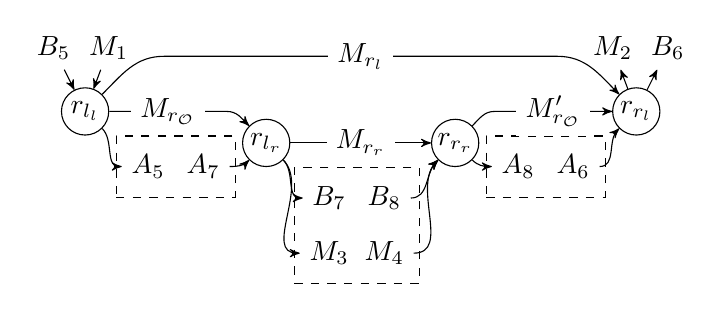
\begin{tikzpicture}[on grid]
        \node[vert] (ll) at (0, 0) {$r_{l_l}$};
        \node[vert, right=2.3 of ll, yshift=-4mm] (lr) {$r_{l_r}$};
        \node[vert, right=7 of ll] (rr) {$r_{r_l}$};
        \node[vert, left=2.3 of rr, yshift=-4mm] (rl) {$r_{r_r}$};

        \node (A1) [above left=0.8 and 0.4 of ll] {$B_5$};
        \node (A2) [above right=0.8 and 0.4 of rr] {$B_6$};
        \node (A3) [below right=0.7 and 0.8 of lr] {$B_7$};
        \node (A4) [right=0.7 of A3] {$B_8$};

        \node (B1) [below right=0.7 and 0.8 of ll] {$A_5$};
        \node (B3) [right=0.7 of B1] {$A_7$};
        \node (B2) [below left=0.7 and 0.8 of rr] {$A_6$};
        \node (B4) [left=0.7 of B2] {$A_8$};

        \node (M1) [right=0.7 of A1] {$M_1$};
        \node (M2) [left=0.7 of A2] {$M_2$};
        \node (M3) [below=0.7 of A3] {$M_3$};
        \node (M4) [below=0.7 of A4] {$M_4$};

        \node[draw,dashed,fit=(B1) (B3), inner xsep = 2pt] (box1) {};
        \node[draw,dashed,fit=(A3) (A4) (M3) (M4), inner xsep = 2pt] (box2) {};
        \node[draw,dashed,fit=(B2) (B4), inner xsep = 2pt] (box3) {};

        \draw [->] (A1) -- (ll);
        \draw [->] (rr) -- (A2);
        \draw [->] (M1) -- (ll);
        \draw [->] (rr) -- (M2);

        \draw [->] (ll) -- ++(1.8,0) node[midway, fill=white] {$M_{r_\mathcal{O}}$} to[out=east, in=north west] (lr);
        \draw [->] (ll) to[out=south east,in=west] (B1);
        \draw [->] (B3) to[out=east,in=south west] (lr);

        \draw [->] (lr) -- node[midway, fill=white] {$M_{r_r}$} (rl);
        \draw [->] (lr) to[out=south east,in=west] (A3);
        \draw [->] (lr) to[out=south east,in=west] (M3);
        \draw [->] (A4) to[out=east,in=south west] (rl);
        \draw [->] (M4) to[out=east,in=south west] (rl);

        \draw [->] (rl) to[out=north east, in=west] ($(rr)-(1.8,0)$) -- node[midway, fill=white] {$M_{r_\mathcal{O}}^\prime$} (rr);
        \draw [->] (rl) to[out=south east,in=west] (B4);
        \draw [->] (B2) to[out=east,in=south west] (rr);

        \draw[->] (ll) to[out=north east, in=west] ++(1,0.7)
         -- ++(5,0) node[midway,fill=white] {$M_{r_l}$}
         to[out=east, in=north west] (rr)
        ;
    \end{tikzpicture}
\end{equation}

Now, writing down the 3-optic is simply a matter of matching up the $M$s, and
setting corresponding gaps opposite each other. This is done in figure \ref{fig:3optic}.
Additionally, the composition rule for 3 optics is shown in the appendix in figure
\ref{fig:3opticcomp}.

\begin{figure*}
\begin{center}
    \begin{tikzpicture}[on grid]
        \node[vert] (lll) at (0, 0) {$l_{l_l}$};
        \node[vert, right=2.3 of lll, yshift=-4mm] (rll) {$r_{l_l}$};
        \node[vert, right=2.3 of rll, yshift=-4mm] (rlr) {$r_{l_r}$};
        \node[vert, right=2.3 of rlr, yshift=-4mm] (llr) {$l_{l_r}$};

        \node[vert, right=16 of ll] (lrl) {$l_{r_l}$};
        \node[vert, left=2.3 of lrl, yshift=-4mm] (rrl) {$r_{r_l}$};
        \node[vert, left=2.3 of rrl, yshift=-4mm] (rrr) {$r_{r_r}$};
        \node[vert, left=2.3 of rrr, yshift=-4mm] (lrr) {$l_{r_r}$};

        \node (A1) [left=0.8 of lll] {$A_1$};
        \node (A2) [right=0.8 of lrl] {$A_2$};

        \node (B1) [below right=0.7 and 0.75 of lll] {$B_1$};
        \node (B5) [right=0.7 of B1] {$B_5$};

        \node (A5) [below right=0.7 and 0.75 of rll] {$A_5$};
        \node (A7) [right=0.7 of A5] {$A_7$};

        \node (B7) [below right=0.7 and 0.75 of rlr] {$B_7$};
        \node (B3) [right=0.7 of B7] {$B_3$};

        \node (A3) [below right=0.7 and 0.75 of llr] {$A_3$};
        \node (A4) [right=0.7 of A3] {$A_4$};

        \node (B8) [below left=0.7 and 0.8 of rrr] {$B_8$};
        \node (B4) [left=0.7 of B8] {$B_4$};

        \node (A6) [below left=0.7 and 0.8 of rrl] {$A_6$};
        \node (A8) [left=0.7 of A6] {$A_8$};

        \node (B2) [below left=0.7 and 0.8 of lrl] {$B_2$};
        \node (B6) [left=0.7 of B2] {$B_6$};

        \node[draw,dashed,fit=(B1) (B5), inner xsep = 2pt] (box1) {};
        \node[draw,dashed,fit=(A5) (A7), inner xsep = 2pt] (box2) {};
        \node[draw,dashed,fit=(B7) (B3), inner xsep = 2pt] (box3) {};
        \node[draw,dashed,fit=(A3) (A4), inner xsep = 2pt] (box4) {};
        \node[draw,dashed,fit=(B4) (B8), inner xsep = 2pt] (box5) {};
        \node[draw,dashed,fit=(A8) (A6), inner xsep = 2pt] (box6) {};
        \node[draw,dashed,fit=(B6) (B2), inner xsep = 2pt] (box7) {};


        \draw [->] (A1) -- (lll);
        \draw [->] (lrl) -- (A2);

        \foreach \s/\t/\l in {lll/rll/$M_{1}$,
                              rll/rlr/$M_{r_{\mathcal{O}}}$,
                              rlr/llr/$M_{3}$} {
            \draw [->] (\s) -- ++(1.8,0) node[midway, fill=white] {\l} to[out=east, in=north west] (\t);
        }

        \foreach \s/\t/\l in {lrr/rrr/$M_{4}$,
                              rrr/rrl/$M_{r_{\mathcal{O}}}^\prime$,
                              rrl/lrl/$M_{2}$} {
            \draw [->] (\s) to[out=north east, in=west] ($(\t)-(1.8,0)$) -- node[midway, fill=white] {\l} (\t);
        }

        \draw[->] (rll) to[out=north east, in=west] ++(1,0.5)
         -- ++(9.5,0) node[midway,fill=white] {$M_{r_l}$}
         to[out=east, in=north west] (rrl)
        ;

        \draw[->] (rlr) to[out=north east, in=west] ++(1,0.4)
        -- ++(5,0) node[midway,fill=white] {$M_{r_r}$}
        to[out=east, in=north west] (rrr)
       ;


        \draw[->] (lll) to[out=north east, in=west] ++(1,0.9)
         -- ++(14,0) node[midway,fill=white] {$M_{l_l}$}
         to[out=east, in=north west] (lrl)
        ;

        \draw[->] (lll) to[out=north east, in=west] ++(1,0.5)
         -- ++(4,0) node[midway,fill=white] {$M_{l_\mathcal{O}}$}
         to[out=east, in=north west] (llr)
        ;

        \draw[->] (llr) -- (lrr) node[midway,fill=white] {$M_{l_r}$};

        \draw [->] (lrr) to[out=north east, in=west] ($(lrl)-(5,-0.5)$) -- ++(4,0) node[midway, fill=white] {$M_{l_\mathcal{O}}^\prime$} to[out=east, in=north west] (lrl);

        \foreach \s/\t in {lll/B1, rll/A5, rlr/B7, llr/A3, lrr/B4, rrr/A8, rrl/B6} {
            \draw[->] (\s) to[out=south east, in=west] (\t);
        }

        \foreach \s/\t in {B5/rll, A7/rlr, B3/llr, A4/lrr, B8/rrr, A6/rrl, B2/lrl} {
            \draw[->] (\s) to[out=east, in=south west] (\t);
        }

    \end{tikzpicture}
\end{center}
\caption{Wiring diagram for the canonical 3-optic $(A_{1-8}) \hto (B_{1-8})$}
\label{fig:3optic}
\end{figure*}

\subsection{Well-behaved primitives}

We say a primitive of an optic functor $\euro$ is \textit{well behaved} if the
LHS of $\euro f$ is simply the original function `f', possibly with a capture
of the input or output value, i.e. $\euro f = \langle \Delta_{SSA} \bbsemi
(id \otimes f) | f^\star \rangle$ or $\euro f = \langle f \bbsemi \Delta_{SSA} | f^\star \rangle$.
For functions of this form, various higher order concepts simplify and we can
perform analysis efficiently using dynamic programming. Speciafically, for an
order $n$ transform, we only need to do $n^2 - 1$ work rather than $2^n$ as would
naively be expected. To see this, note that by repeatedly applying the transform,
we can commute any function in our $n$-optic to just be a structural transform
together with $f^{\star\star\ldots}$ where the number of stars is the total
number of stars in the original expression. Then, letting numbers indicate
the number of stars, we get the following sequence of patterns for
increasing optics: $0$, $01$, $0121$, $01212321$, $0121232123432321$, which
is amenable to dynamic programming analysis.

\todo[inline]{Is this actually a useful notion? Certainly more advanced. Let's leave it here
for now.}

\section{Reverse mode AD}

There are many ways to describe the difference between forward and reverse mode
AD, but using our newfound language, it becomes quite simple: Forward mode AD
pushes forward tangent vectors, while reverse mode AD pulls back cotangent vectors.

Now for the payoff from all of our hard work from the previous sections: Computing
pullbacks of differential forms has the structure of an optic. As a concrete
example, suppose we wanted to compute the gradient $\nabla f$. Tracing through our
definitions above, we find that:

\begin{equation}
\nabla f (x) = f^\star(dx_1(f(x)))
\end{equation}

so two evaluate this function we first have a covariant evaluation of $f$,
followed by a contravariant evaluation of $f^\star$. Now for the formal construction:
Let $\mathcal{C}$ be the category of Riemannian manifolds. We have an optic
category $\Optic_{\mathcal{C}}(T^\star M)$
\footnote{We're cheating here a little bit by calling the pair $(A,A^\prime)$ simply $T^\star M$,
technically we have a dependent optic $(x: M, T_x M)$, but since our programming
language does not care about such things, we're happy to cheat an let others work out the tedious details.}
that pairs to each manifold its
tangent bundle. Now, guided by the above, we defined a functor:

\begin{equation}
\overleftarrow{\partial} f: \mathcal{C} \to \Optic_{\mathcal{C}}(T^\star M)
\end{equation}

where as indicated, $\overleftarrow{\partial} M = T^\star M$ and on morphisms
$\overleftarrow{\partial} f = \langle (a\to(a,f(a)), (a, z) \to f^\star|_{a}(z) \rangle$.

We call this functor the \textbf{Reverse mode AD optic functor}.

There is very little left to do at this point, but our program above did teach
us that we need to define a few things:

For copy, we simply write
\begin{equation}
\overleftarrow{\partial} copy(x) = (x, x), (\Delta_1, \Delta_2) \to \Delta_1 + \Delta_2
\end{equation}
which is the unique map that preserves linear of the pullback. For delete:
\begin{equation}
    \overleftarrow{\partial} delete(x) = ()\to 0
\end{equation}
For branch we have a choice. We could either inherit the behavior from delete
or return a poison value on the backwards pass. This is a user level policy decision.

Lastly, we of course need to define derivatives for our primitives. We defer
this task to ChainRules.jl.

\section{Higher order AD}

\subsection{Straightforwardly}

Let us investigate the structure of higher order AD.
One straightforward way to obtain the higher order transform is to simply
treat the encoded optic as yet another SSA program.
As an example, we may explicitly do the transform $\overleftarrow{\partial} \overleftarrow{\partial} \text{sin}$:

\begin{snippet}
function |$\overleftarrow{\partial} \overleftarrow{\partial}$|sin(x)
    sin(x), |$\Delta$|->begin
        |$\Delta$| * cos(x), |$\Delta'$|->begin
            |$\Delta'$|*|$\Delta$|*(-sin(x)), |$\Delta'$|*cos(x)
        end
    end, (|$\Delta'''$|,|$\Delta''$|)->begin
        |$\Delta''$|*cos(x) + |$\Delta'''$|
    end
end
\end{snippet}

Recall from above the diagram for an optic functor

\begin{equation}
    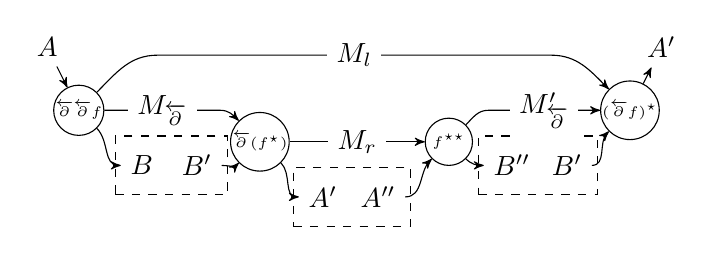
\begin{tikzpicture}[on grid]
        \node[vert] (ll) at (0, 0) {\tiny{$\overleftarrow{\partial} \overleftarrow{\partial} f$}};
        \node[vert, right=2.3 of ll, yshift=-4mm] (lr) {\tiny{$\overleftarrow{\partial}(f^\star)$}};
        \node[vert, right=7 of ll] (rr) {\tiny{$(\overleftarrow{\partial} f)^\star$}};
        \node[vert, left=2.3 of rr, yshift=-4mm] (rl) {\tiny{$f^{\star\star}$}};

        \node (A1) [above left=0.8 and 0.4 of ll] {$A$};
        \node (A2) [above right=0.8 and 0.4 of rr] {$A'$};

        \node (B1) [below right=0.7 and 0.8 of ll] {$B$};
        \node (B3) [right=0.7 of B1] {$B'$};

        \node (A3) [below right=0.7 and 0.8 of lr] {$A'$};
        \node (A4) [right=0.7 of A3] {$A''$};

        \node (B2) [below left=0.7 and 0.8 of rr] {$B'$};
        \node (B4) [left=0.7 of B2] {$B''$};

        \node[draw,dashed,fit=(B1) (B3), inner xsep = 2pt] (box1) {};
        \node[draw,dashed,fit=(A3) (A4), inner xsep = 2pt] (box2) {};
        \node[draw,dashed,fit=(B2) (B4), inner xsep = 2pt] (box3) {};

        \draw [->] (A1) -- (ll);
        \draw [->] (rr) -- (A2);

        \draw [->] (ll) -- ++(1.8,0) node[midway, fill=white] {$M_{\overleftarrow{\partial}}$} to[out=east, in=north west] (lr);
        \draw [->] (ll) to[out=south east,in=west] (B1);
        \draw [->] (B3) to[out=east,in=south west] (lr);

        \draw [->] (lr) -- node[midway, fill=white] {$M_r$} (rl);
        \draw [->] (lr) to[out=south east,in=west] (A3);
        \draw [->] (A4) to[out=east,in=south west] (rl);

        \draw [->] (rl) to[out=north east, in=west] ($(rr)-(1.8,0)$) -- node[midway, fill=white] {$M_{\overleftarrow{\partial}}^\prime$} (rr);
        \draw [->] (rl) to[out=south east,in=west] (B4);
        \draw [->] (B2) to[out=east,in=south west] (rr);

        \draw[->] (ll) to[out=north east, in=west] ++(1,0.7)
         -- ++(5,0) node[midway,fill=white] {$M_l$}
         to[out=east, in=north west] (rr)
        ;
    \end{tikzpicture}
\end{equation}

We can identify the various arrows with concrete values in the program:

\begin{center}
\begin{tabular}{c|c}
Diagram & Program \\ \hline
$M_l$ & Capture of $x$ in the last closure \\
$ M_{\overleftarrow{\partial}} $ & Capture of x in the first closure \\
B & Return value of $\overleftarrow{\partial} \overleftarrow{\partial} \text{sin}$ \\
$B'$ & $\Delta$ \\
$M_r$ & Capture of $\Delta$, $x$ by the inner closure \\
$A'$ & Primal return value of the first closure ($\Delta * \text{cos}(x)$) \\
$A''$ & $\Delta'$ \\
$B''$ & Second return, inner closure ($\Delta' * \text{cos}(x)$) \\
$M_{\overleftarrow{\partial}}'$ & First return, inner closure ($- \Delta' * \Delta * \text{sin}(x)$) \\
& Also, $\Delta'''$ \\
$B'$ & $\Delta''$
\end{tabular}
\end{center}

In particular, if we are taking the second derivative of sin, here is the
dataflow path of the final answer:

\begin{equation}
    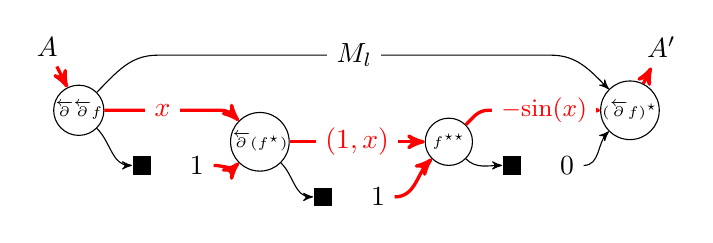
\begin{tikzpicture}[on grid]
        \node[vert] (ll) at (0, 0) {\tiny{$\overleftarrow{\partial} \overleftarrow{\partial} f$}};
        \node[vert, right=2.3 of ll, yshift=-4mm] (lr) {\tiny{$\overleftarrow{\partial}(f^\star)$}};
        \node[vert, right=7 of ll] (rr) {\tiny{$(\overleftarrow{\partial} f)^\star$}};
        \node[vert, left=2.3 of rr, yshift=-4mm] (rl) {\tiny{$f^{\star\star}$}};

        \node (A1) [above left=0.8 and 0.4 of ll] {$A$};
        \node (A2) [above right=0.8 and 0.4 of rr] {$A'$};

        \node (B1) [below right=0.7 and 0.8 of ll,fill=black] {};
        \node (B3) [right=0.7 of B1] {$1$};

        \node (A3) [below right=0.7 and 0.8 of lr, fill=black] {};
        \node (A4) [right=0.7 of A3] {$1$};

        \node (B2) [below left=0.7 and 0.8 of rr] {$0$};
        \node (B4) [left=0.7 of B2, fill=black] {};

        \draw [->,color=red, very thick] (A1) -- (ll);
        \draw [->,color=red, very thick] (rr) -- (A2);

        \draw [->,color=red, very thick] (ll) -- ++(1.8,0) node[midway, fill=white] {$x$} to[out=east, in=north west] (lr);
        \draw [->] (ll) to[out=south east,in=west] (B1);
        \draw [->,color=red, very thick] (B3) to[out=east,in=south west] (lr);

        \draw [->,color=red, very thick] (lr) -- node[midway, fill=white] {$(1,x)$} (rl);
        \draw [->] (lr) to[out=south east,in=west] (A3);
        \draw [->,color=red, very thick] (A4) to[out=east,in=south west] (rl);

        \draw [->,color=red, very thick] (rl) to[out=north east, in=west] ($(rr)-(1.8,0)$) -- node[midway, fill=white] {\small{$-\text{sin}(x)$}} (rr);
        \draw [->] (rl) to[out=south east,in=west] (B4);
        \draw [->] (B2) to[out=east,in=south west] (rr);

        \draw[->] (ll) to[out=north east, in=west] ++(1,0.7)
         -- ++(5,0) node[midway,fill=white] {$M_l$}
         to[out=east, in=north west] (rr)
        ;
    \end{tikzpicture}
\end{equation}

For a more complex example, the same transform is done for a third order
transform in the Appendix (figure \ref{3-ordernaive}).

\subsection{Alternative encoding}

The previous approach works, but it is somewhat unsatisfying. Why? For me the two
primary reasons are that there is no manifest difference between the residuals
and the "holes" of the optic and that control flow is somewhat non-transparent.
At first order, the residual was encoded as the
capture of the original closure. However, at second order, while most residuals
are still closure captures, $\Delta^{\prime\prime}$ is a residual, but does not
look like a capture. This shows up more at third order. To see what I mean
when I say control-flow is non-transparent, consider the order in which the
functions are called at third order:
\newcommand{\op}{\overleftarrow{\partial}}

\begin{equation}
\begin{split}
\op\op f, \op \op \left( f^\star \right), \op \left( f^{\star\star} \right), \op \left( \left( \op f\right)^{\star} \right), \\
\left( \op f\right)^{\star\star}, f^{\star\star\star}, \left( \op \left( f^\star \right) \right)^{\star}, \left( \op \op f\right)^{\star}
\end{split}
\end{equation}

(if it's not clear how to come up with this order, simply look at the second
order diagram, add $\op$ in front of everything, then reverse the diagram,
add $\star$ after everything and append the reversed diagram to the one that
had $\op$ added). Comparing this to figure \ref{3-ordernaive} in the appendix,
we see that in source code order, the sequence is $1,2,3,6,7,5,8$, so we need
to do a lot of jumping around to keep track of what's happening.
Can we re-arrange the encoding to make it easier to understand what's going on?
Let's take a clue from the diagrams we've been working with, which do make the
control flow order manifestly clear. What if instead of our second order example
above, we wrote it as:

\begin{snippet}
function |$\partial^2$|sin(x)
    sin(x), |$\Delta$|->begin
        |$\Delta$| * cos(x), |$\Delta'$|->begin
            |$\Delta'$|*cos(x), let |$\Delta'''$| = |$\Delta'$|*|$\Delta$|*(-sin(x))
                |$\Delta''$|->|$\Delta''$|*cos(x) + |$\Delta'''$|
            end
        end
    end
end
\end{snippet}

This avoids the two problems identified above: The $\Delta'''$ becomes an
explicit capture and the order of operations becomes quite clear
(outer functions are evaluated before their inner closures). This representation
is a bit of a re-think of the standard transform, but it is entirely equivalent.
To get more familiar with it, let's say, we'd like to take the third order transform
of the following functions:

\begin{snippet}
function f(x)
    y = g(x)
    z = h(y)
    return z
end
\end{snippet}

We would have:


\begin{snippet}
function |$\op^3$|f(x)
  |$y$|, |$\overline{y}$| = |$\op^3$|g(x)
  |$z$|, |$\overline{z}$| = |$\op^3$|h(y)
  |$z$|, |$\Delta$|->begin
    |$\alpha$|, |$\overline{\alpha}$| = |$\overline{z}$|(|$\Delta$|)
    |$\beta$|, |$\overline{\beta}$| = |$\overline{y}$|(|$\alpha$|)
    |$\beta$|, |$\Delta'$|->begin
      |$\gamma$|, |$\overline{\gamma}$| = |$\overline{\beta}$|(|$\Delta'$|)
      |$\delta$|, |$\overline{\delta}$| = |$\overline{\alpha}$|(|$\gamma$|)
      |$\delta$|, |$\Delta''$|->begin
        |$\epsilon$|, |$\overline{\epsilon}$| = |$\overline{\delta}$|(|$\Delta''$|)
        |$\zeta$|, |$\overline{\zeta}$| = |$\overline{\gamma}$|(|$\epsilon$|)
        |$\zeta$|, |$\Delta'''$|->begin
          |$\eta$|, |$\overline{\eta}$| = |$\overline{\zeta}$|(|$\Delta'''$|)
          |$\theta$|, |$\overline{\theta}$| = |$\overline{\epsilon}$|(|$\eta$|)
          |$\theta$|, |$\Delta^4$|->begin
            |$\iota$|, |$\overline{\iota}$| = |$\overline{\theta}$|(|$\Delta^4$|)
            |$\kappa$|, |$\overline{\kappa}$| = |$\overline{\eta}$|(|$\iota$|)
            |$\kappa$|, |$\Delta^5$|->begin
              |$\lambda$|, |$\overline{\lambda}$| = |$\overline{\kappa}$|(|$\Delta^5$|)
              |$\mu$|, |$\overline{\mu}$| = |$\overline{\iota}$|(|$\lambda$|)
              |$\mu$|, |$\Delta^6$|->begin
                |$\nu$|, |$\overline{\nu}$| = |$\overline{\mu}$|(|$\Delta^6$|)
                |$\xi$|, |$\overline{\xi}$| = |$\overline{\lambda}$|(|$\nu$|)
                |$\xi$|, |$\Delta^7$|->begin
                  |$o$| = |$\overline{\xi}$|(|$\Delta^7$|)
                  |$\pi$| = |$\overline{\nu}$|(|$o$|)
                  return |$\pi$|
                end
              end
            end
          end
        end
      end
    end
  end
end
\end{snippet}

We see still have the same number of functions, so the complexity isn't
reduced, but at least it's fairly orderly. We do have to take special care of
primitives, because we're no longer just applying the same transformation to
the rule function itself. So suppose we have some primitive rule like:

\begin{snippet}
struct |$\nabla a$|
    x
end
(::|$\nabla a$|) = ...

function rrule(::typeof(a), x)
    b(x), |$\nabla a$|(x)
end

\end{snippet}

For the first order, we would just expose the raw pullback as we do with
the naive transform. However, for second order, things become slightly more
complicated:


\begin{snippet}
function |$\op^2 a$|(x)
    (|$y$|, |$\overline{y}$|), |$\overline{\overline{y}}$| = |$\op \text{rrule}$|(a, x)
    |$y$|, |$\Delta$|->begin
        |$\alpha$|, |$\overline{\alpha}$| = |$\op \text{typeof(}\overline{y}\text{)}$|(|$\overline{y}$|, |$\Delta$|)
        |$\alpha$|, |$\Delta'$|->begin
            (|$\Delta'''$|, |$\beta$|) = |$\overline{\alpha}$|(|$\Delta'$|)
            |$\beta$|, |$\Delta''$|->begin
                # Drop gradient w.r.t. `rrule`
                (_, a', x') = |$\overline{\overline{y}}$|(|$\Delta''$|, |$\Delta'''$|)
                return (a', x')
            end
        end
    end
end
\end{snippet}

It's worth comparing this with the explicitly written out and inlined version of
sin above (which is a primitive).

It's also worth taking a look at the third order version of that example to see
the generalizing pattern:

\begin{snippet}
function |$\op^3 a$|(x)
    (|$y$|, |$\overline{y}$|), |$\overline{\overline{y}}$| = |$\op^2 \text{rrule}$|(a, x)
    |$y$|, |$\Delta$|->begin
        (|$\alpha$|, |$\overline{\alpha}$|) = |$\op^2 \text{typeof(}\overline{y}\text{)}$|(|$\overline{y}$|, |$\Delta$|)
        |$\alpha$|, |$\Delta'$|->begin
            (|$\Delta'''$|, |$\beta$|), |$\overline{\beta}$| = |$\overline{\alpha}$|(|$\Delta'$|)
            |$\beta$|, |$\Delta''$|->begin
                (_, |$\gamma_1$|, |$\gamma_2$|), |$\overline{\gamma}$| = |$\overline{\overline{y}}$|(|$\Delta''$|, |$\Delta'''$|)
                (|$\gamma_1$|, |$\gamma_2$|), |$\Delta^4$|->begin
                    (|$\delta_1$|, |$\delta_2$|), |$\overline{\delta}$| = |$\overline{\gamma}$|((0, |$\Delta^4$|...))
                    |$\delta_1$|, |$\Delta^5$|->begin
                        |$\epsilon$|, |$\overline{\epsilon}$| = |$\overline{\beta}$|(|$\delta_2$|, |$\Delta^5$|)
                        |$\epsilon$|, |$\Delta^6$|->begin
                            (|$\zeta_1$|, |$\zeta_2$|)  = |$\overline{\epsilon}$|(|$\Delta^6$|)
                            |$\zeta_2$|, |$\Delta^7$|->begin
                                return |$\overline{\delta}$|(|$\Delta^7$|, |$\zeta_1$|)
                            end
                        end
                    end
                end
            end
        end
    end
end
\end{snippet}

If this structure seems familiar, it should! In our $3$-optic diagram we
build $3$-optics as pairs of $2$-optics that composed in a canonical way.
This is just the very same thing (compare functions $l_{x_{x}}$ with
closures returned from $\op^2 \text{rrule}$ and $r_{x_{x}}$ with
closures returned from $\op^2 \text{typeof(}\overline{y}\text{)}$).

There is one additional case that's worth considering: We allow explicitly
calling the derivative operator in the primal. What happens when we encounter
such a function. The answer is fairly straightforward. We're basically doing
the inverse of the rrule case above. In particular, we're adapting an $n+1$
optic to an $n$ optic by appropriate interleaving. Suppose we have a primal
function $\nabla$ given by:

\begin{snippet}
function |$\nabla$|(f, x)
    (|$a$|, |$\overline{a}$|) = |$\op$|(f, x)
    |$y$| = g(a)
    |$z$| = |$\overline{a}$|(y)
    return |$z$|
end
\end{snippet}

Applying our transform, we get:

\begin{snippet}
function |$\op\nabla$|(f, x)
    (|$a$|, |$\overline{a}$|) = |$\op^2$|(f, x)
    |$y$|, |$\overline{y}$| = |$\op g$|(a)
    |$z$|, |$\overline{z}$| = |$\overline{a}$|(y)
    |$z$|, |$\Delta$|->begin
        |$\alpha$|, |$\overline{\alpha}$| = |$\overline{z}$|(|$\Delta$|)
        |$\beta$| = |$\overline{y}$|(|$\alpha$|)
        |$\epsilon$| = |$\overline{\alpha}$|(|$\beta$|)
        return |$\epsilon$|
    end
end
\end{snippet}

Note that we went through all four callbacks of the $2$-optic $\op^2(f, x)$,
even though the top level optic only had two callbacks. For completeness,
here is the third order version (second order transform):

\begin{snippet}
function |$\op^2\nabla$|(f, x)
    (|$a$|, |$\overline{a}$|) = |$\op^3$|(f, x)
    |$y$|, |$\overline{y}$| = |$\op g$|(a)
    |$z$|, |$\overline{z}$| = |$\overline{a}$|(y)
    |$z$|, |$\Delta$|->begin
        |$\alpha$|, |$\overline{\alpha}$| = |$\overline{z}$|(|$\Delta$|)
        |$\beta$|, |$\overline{\beta}$| = |$\overline{y}$|(|$\alpha$|)
        |$\epsilon$|, |$\overline{\beta}$| = |$\overline{\alpha}$|(|$\beta$|)
        |$\epsilon$|, |$\Delta'$|->begin
            |$\lambda$|, |$\overline{\lambda}$| = |$\overline{\epsilon}$|(|$\Delta'$|)
            |$\zeta$|, |$\overline{\zeta}$| = |$\overline{\beta}$|(|$\lambda$|)
            |$\mu$|, |$\overline{\mu}$| = |$\overline{\lambda}$|(|$\zeta$|)
            |$\mu$|, |$\Delta''$|->begin
                |$\theta$|, |$\overline{\theta}$| = |$\overline{\mu}$|(|$\Delta''$|)
                |$\iota$| = |$\overline{\zeta}$|(|$\theta$|)
                |$\kappa$| = |$\overline{\theta}$|(|$\iota$|)
                return |$\kappa$|
            end
        end
    end
end
\end{snippet}

\section{Implementation details}

The key to a performant reverse mode AD implementation is to pick
efficient residual representatives $M$ for our optic as well as introducing
minimal additional overhead in the tensor. In julia, the latter means
being amenable to type inference (as well as ideally not being significantly harder
on type inference than a simple primal inference to avoid unexpected performance
cliffs). So, how do perform type inference on morphisms from the optic? Well,
if we pick a particular representative, we obtain morphisms in the underlying
category that we can do with whatever we want, including performing inference.
However, picking a representative of course fixes the residual, which we'd like
to avoid. Additionally, we run into problems with nested application of the
functor.

\newpage

\section{Appendix}

Printing the appendix is encouraged to use as a template for working
through examples.

\begin{figure*}
\begin{center}
\scalebox{2}{
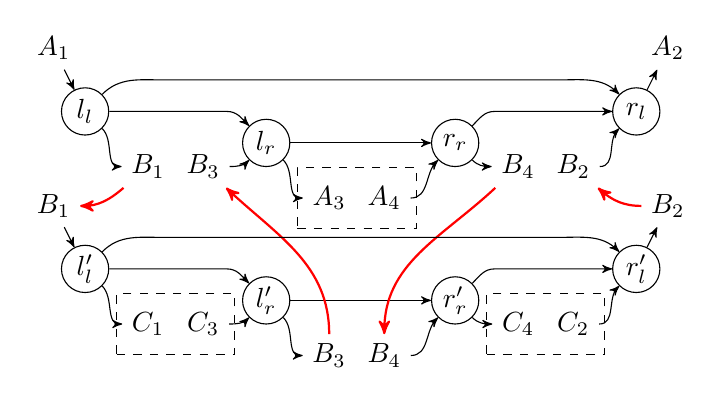
\begin{tikzpicture}[on grid]
    \node[vert] (ll) at (0, 0) {$l_l$};
    \node[vert, right=2.3 of ll, yshift=-4mm] (lr) {$l_r$};
    \node[vert, right=7 of ll] (rr) {$r_l$};
    \node[vert, left=2.3 of rr, yshift=-4mm] (rl) {$r_r$};

    \node (A1) [above left=0.8 and 0.4 of ll] {$A_1$};
    \node (A2) [above right=0.8 and 0.4 of rr] {$A_2$};

    \node (B1) [below right=0.7 and 0.8 of ll] {$B_1$};
    \node (B3) [right=0.7 of B1] {$B_3$};

    \node (A3) [below right=0.7 and 0.8 of lr] {$A_3$};
    \node (A4) [right=0.7 of A3] {$A_4$};

    \node (B2) [below left=0.7 and 0.8 of rr] {$B_2$};
    \node (B4) [left=0.7 of B2] {$B_4$};

    \draw [->] (A1) -- (ll);
    \draw [->] (rr) -- (A2);

    \draw [->] (ll) -- ++(1.8,0) to[out=east, in=north west] (lr);
    \draw [->] (ll) to[out=south east,in=west] (B1);
    \draw [->] (B3) to[out=east,in=south west] (lr);

    \draw [->] (lr) -- (rl);
    \draw [->] (lr) to[out=south east,in=west] (A3);
    \draw [->] (A4) to[out=east,in=south west] (rl);

    \draw [->] (rl) to[out=north east, in=west] ($(rr)-(1.8,0)$) -- (rr);
    \draw [->] (rl) to[out=south east,in=west] (B4);
    \draw [->] (B2) to[out=east,in=south west] (rr);

    \draw[->] (ll) to[out=north east, in=west] ++(1,0.4)
     to ++(5,0)
     to[out=east, in=north west] (rr)
    ;

    \node[draw,dashed,fit=(A3) (A4), inner xsep = 2pt] (box2) {};

    \node[vert, below=2 of ll] (ll_2) {$l_l^\prime$};
    \node[vert, right=2.3 of ll_2, yshift=-4mm] (lr_2) {$l_r^\prime$};
    \node[vert, right=7 of ll_2] (rr_2) {$r_l^\prime$};
    \node[vert, left=2.3 of rr_2, yshift=-4mm] (rl_2) {$r_r^\prime$};

    \node (B1_2) [above left=0.8 and 0.4 of ll_2] {$B_1$};
    \node (B2_2) [above right=0.8 and 0.4 of rr_2] {$B_2$};

    \node (C1) [below right=0.7 and 0.8 of ll_2] {$C_1$};
    \node (C3) [right=0.7 of C1] {$C_3$};

    \node (B3_2) [below right=0.7 and 0.8 of lr_2] {$B_3$};
    \node (B4_2) [right=0.7 of B3_2] {$B_4$};

    \node (C2) [below left=0.7 and 0.8 of rr_2] {$C_2$};
    \node (C4) [left=0.7 of C2] {$C_4$};

    \draw [->] (B1_2) -- (ll_2);
    \draw [->] (rr_2) -- (B2_2);

    \draw [->] (ll_2) -- ++(1.8,0) to[out=east, in=north west] (lr_2);
    \draw [->] (ll_2) to[out=south east,in=west] (C1);
    \draw [->] (C3) to[out=east,in=south west] (lr_2);

    \draw [->] (lr_2) -- (rl_2);
    \draw [->] (lr_2) to[out=south east,in=west] (B3_2);
    \draw [->] (B4_2) to[out=east,in=south west] (rl_2);

    \draw [->] (rl_2) to[out=north east, in=west] ($(rr_2)-(1.8,0)$) -- (rr_2);
    \draw [->] (rl_2) to[out=south east,in=west] (C4);
    \draw [->] (C2) to[out=east,in=south west] (rr_2);

    \draw [->,thick,color=red] (B1)  to[out=south west, in=east] (B1_2);
    \draw [->,thick,color=red] (B3_2) to[out=north, in=south east] (B3);
    \draw [->,thick,color=red] (B4) to[out=south west, in=north] (B4_2);
    \draw [->,thick,color=red] (B2_2) to[out=west, in=south east] (B2);

    \node[draw,dashed,fit=(C1) (C3), inner xsep = 2pt] (box1) {};
    \node[draw,dashed,fit=(C2) (C4), inner xsep = 2pt] (box3) {};

    \draw[->] (ll_2) to[out=north east, in=west] ++(1,0.4)
     to ++(5,0)
     to[out=east, in=north west] (rr_2)
    ;
\end{tikzpicture}

}
\end{center}
\caption{Composition rule for 2-optics (larger version)}
\end{figure*}


\begin{figure*}
    \begin{center}
        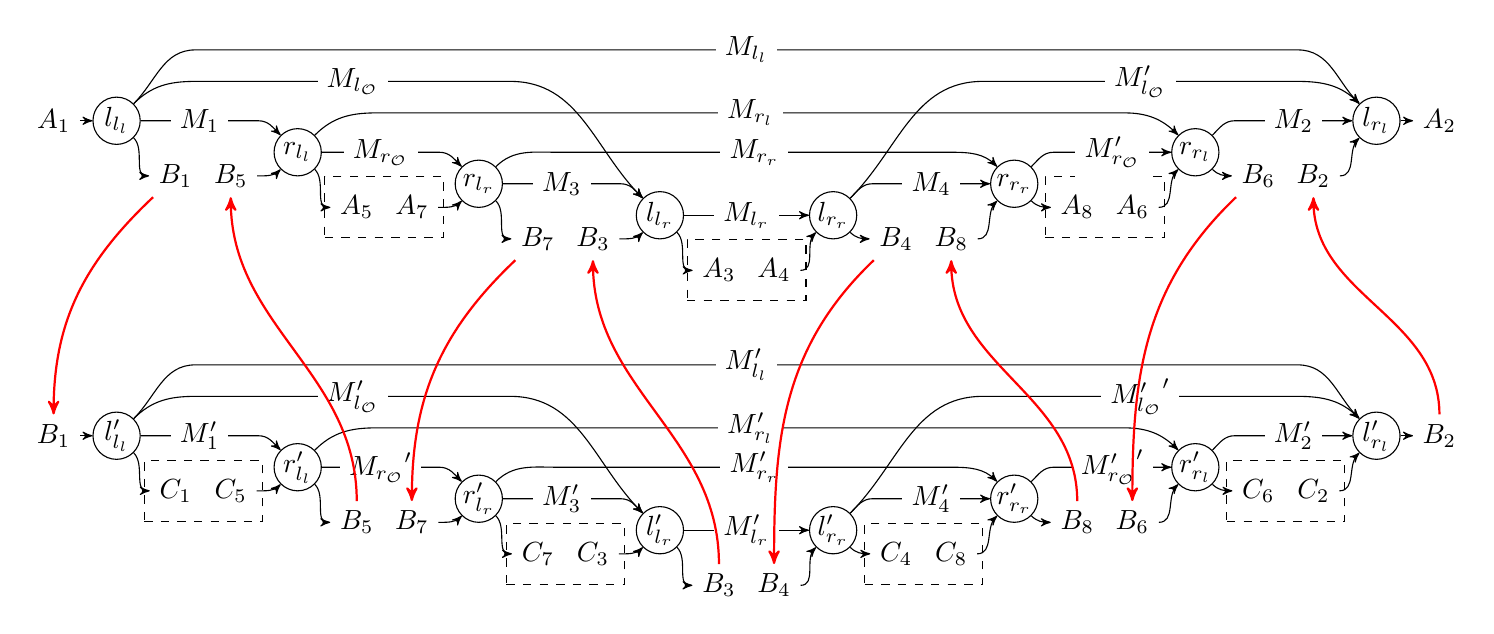
\begin{tikzpicture}[on grid]

        \node[vert] (lll) at (0, 0) {$l_{l_l}$};
        \node[vert, below=4 of lll] (lll') {$l_{l_l}^\prime$};

        \foreach \p in {,'} {
            \newcommand{\A}{\ifdefempty{\p}{A}{B}}
            \newcommand{\B}{\ifdefempty{\p}{B}{C}}

            \node[vert, right=2.3 of lll\p, yshift=-4mm] (rll\p) {$r_{l_l}\p$};
            \node[vert, right=2.3 of rll\p, yshift=-4mm] (rlr\p) {$r_{l_r}\p$};
            \node[vert, right=2.3 of rlr\p, yshift=-4mm] (llr\p) {$l_{l_r}\p$};

            \node[vert, right=16 of lll\p] (lrl\p) {$l_{r_l}\p$};
            \node[vert, left=2.3 of lrl\p, yshift=-4mm] (rrl\p) {$r_{r_l}\p$};
            \node[vert, left=2.3 of rrl\p, yshift=-4mm] (rrr\p) {$r_{r_r}\p$};
            \node[vert, left=2.3 of rrr\p, yshift=-4mm] (lrr\p) {$l_{r_r}\p$};

            \node (A1\p) [left=0.8 of lll\p] {$\A_1$};
            \node (A2\p) [right=0.8 of lrl\p] {$\A_2$};

            \node (B1\p) [below right=0.7 and 0.75 of lll\p] {$\B_1$};
            \node (B5\p) [right=0.7 of B1\p] {$\B_5$};

            \node (A5\p) [below right=0.7 and 0.75 of rll\p] {$\A_5$};
            \node (A7\p) [right=0.7 of A5\p] {$\A_7$};

            \node (B7\p) [below right=0.7 and 0.75 of rlr\p] {$\B_7$};
            \node (B3\p) [right=0.7 of B7\p] {$\B_3$};

            \node (A3\p) [below right=0.7 and 0.75 of llr\p] {$\A_3$};
            \node (A4\p) [right=0.7 of A3\p] {$\A_4$};

            \node (B8\p) [below left=0.7 and 0.8 of rrr\p] {$\B_8$};
            \node (B4\p) [left=0.7 of B8\p] {$\B_4$};

            \node (A6\p) [below left=0.7 and 0.8 of rrl\p] {$\A_6$};
            \node (A8\p) [left=0.7 of A6\p] {$\A_8$};

            \node (B2\p) [below left=0.7 and 0.8 of lrl\p] {$\B_2$};
            \node (B6\p) [left=0.7 of B2\p] {$\B_6$};

            \ifdefempty{\p}{}{
                \node[draw,dashed,fit=(B1\p) (B5\p), inner xsep = 2pt] (box1\p) {};
                \node[draw,dashed,fit=(B7\p) (B3\p), inner xsep = 2pt] (box3\p) {};
                \node[draw,dashed,fit=(B4\p) (B8\p), inner xsep = 2pt] (box5\p) {};
                \node[draw,dashed,fit=(B6\p) (B2\p), inner xsep = 2pt] (box7\p) {};
            };

            \ifdefempty{\p}{
                \node[draw,dashed,fit=(A5\p) (A7\p), inner xsep = 2pt] (box2\p) {};
                \node[draw,dashed,fit=(A3\p) (A4\p), inner xsep = 2pt] (box4\p) {};
                \node[draw,dashed,fit=(A8\p) (A6\p), inner xsep = 2pt] (box6\p) {};
            }{};


            \draw [->] (A1\p) -- (lll\p);
            \draw [->] (lrl\p) -- (A2\p);

            \foreach \s/\t/\l in {lll\p/rll\p/$M_{1}\p$,
                                  rll\p/rlr\p/${M_{r_{\mathcal{O}}}}\p$,
                                  rlr\p/llr\p/$M_{3}\p$} {
                \draw [->] (\s) -- ++(1.8,0) node[midway, fill=white] {\l} to[out=east, in=north west] (\t);
            }

            \foreach \s/\t/\l in {lrr\p/rrr\p/$M_{4}\p$,
                                  rrr\p/rrl\p/${M_{r_{\mathcal{O}}}^\prime}\p$,
                                  rrl\p/lrl\p/$M_{2}\p$} {
                \draw [->] (\s) to[out=north east, in=west] ($(\t)-(1.8,0)$) -- node[midway, fill=white] {\l} (\t);
            }

            \draw[->] (rll\p) to[out=north east, in=west] ++(1,0.5)
             -- ++(9.5,0) node[midway,fill=white] {$M_{r_l}\p$}
             to[out=east, in=north west] (rrl\p)
            ;

            \draw[->] (rlr\p) to[out=north east, in=west] ++(1,0.4)
            -- ++(5,0) node[midway,fill=white] {$M_{r_r}\p$}
            to[out=east, in=north west] (rrr\p)
           ;


            \draw[->] (lll\p) to[out=north east, in=west] ++(1,0.9)
             -- ++(14,0) node[midway,fill=white] {$M_{l_l}\p$}
             to[out=east, in=north west] (lrl\p)
            ;

            \draw[->] (lll\p) to[out=north east, in=west] ++(1,0.5)
             -- ++(4,0) node[midway,fill=white] {$M_{l_\mathcal{O}}\p$}
             to[out=east, in=north west] (llr\p)
            ;

            \draw[->] (llr\p) -- (lrr\p) node[midway,fill=white] {$M_{l_r}\p$};

            \draw [->] (lrr\p) to[out=north east, in=west] ($(lrl\p)-(5,-0.5)$) -- ++(4,0) node[midway, fill=white] {${M_{l_\mathcal{O}}^\prime}\p$} to[out=east, in=north west] (lrl\p);

            \foreach \s/\t in {lll/B1, rll/A5, rlr/B7, llr/A3, lrr/B4, rrr/A8, rrl/B6} {
                \draw[->] (\s\p) to[out=south east, in=west] (\t\p);
            }

            \foreach \s/\t in {B5/rll, A7/rlr, B3/llr, A4/lrr, B8/rrr, A6/rrl, B2/lrl} {
                \draw[->] (\s\p) to[out=east, in=south west] (\t\p);
            }
        }

        \draw [->,thick,color=red] (B1) to[out=south west, in=north] (A1');
        \draw [->,thick,color=red] (B7) to[out=south west, in=north] (A7');
        \draw [->,thick,color=red] (B4) to[out=south west, in=north] (A4');
        \draw [->,thick,color=red] (B6) to[out=south west, in=north] (A6');

        \draw [->,thick,color=red] (A5') to[out=north, in=south] (B5);
        \draw [->,thick,color=red] (A3') to[out=north, in=south] (B3);
        \draw [->,thick,color=red] (A8') to[out=north, in=south] (B8);
        \draw [->,thick,color=red] (A2') to[out=north, in=south] (B2);

    \end{tikzpicture}
    \end{center}
    \caption{Composition rule for 3-optics}
    \label{fig:3opticcomp}
\end{figure*}

\begin{figure*}
\begin{minted}[fontsize=\huge, framesep=2mm,escapeinside=||,mathescape=true,frame=lines,linenos]{julia}
function |$\overleftarrow{\partial} \overleftarrow{\partial}$|sin(x)
    sin(x), |$\Delta$|->begin
        |$\Delta$| * cos(x), |$\Delta'$|->begin
            |$\Delta'$|*|$\Delta$|*(-sin(x)), |$\Delta'$|*cos(x)
        end
    end, (|$\Delta'''$|,|$\Delta''$|)->begin
        |$\Delta''$|*cos(x) + |$\Delta'''$|
    end
end
\end{minted}
\caption{Explicitly written 2-nd order example (larger version)}
\end{figure*}

\begin{figure*}
\begin{minted}[framesep=2mm,escapeinside=||,mathescape=true,frame=lines,linenos]{julia}
function |$\overleftarrow{\partial} \overleftarrow{\partial} \overleftarrow{\partial}$|sin(x)
    (sin(x), |$\Delta$|->begin # $\overleftarrow{\partial} \overleftarrow{\partial} (f^{\star})$
        |$\Delta$| * cos(x), |$\Delta'$|->begin # $\overleftarrow{\partial} (f^{\star\star})$
            |$\Delta'$|*|$\Delta$|*(-sin(x)), |$\Delta'$|*cos(x), ((|$\Delta^4$|,|$\Delta^5$|),)->begin # $ f^{\star\star\star} $
                (-|$\Delta^4$|*|$\Delta'$|*|$\Delta$|*cos(x) +
                    -|$\Delta^5$|*|$\Delta'$|*sin(x),
                    -|$\Delta^4$|*|$\Delta'$|*sin(x)),
                -|$\Delta^4$|*|$\Delta$|*sin(x)+|$\Delta^5$|*cos(x)
            end
        end, (|$\Delta^6$|,(|$\Delta^7$|,|$\Delta^8$|))->begin # $ \left(\overleftarrow{\partial}\left(f^\star\right)\right)^{\star} $
            (|$\Delta^6$|*|$\Delta$|*(-sin(x)) + |$\Delta^7$|,
                |$\Delta^6$|*cos(x) + |$\Delta^8$|)
        end
    end, (|$\Delta'''$|,|$\Delta''$|)->begin # $ \overleftarrow{\partial} \left( \left( \overleftarrow{\partial} f \right)^\star \right)  $
        |$\Delta''$|*cos(x) + |$\Delta'''$|, |$\Delta^9$|->begin # $ \left( \overleftarrow{\partial} f \right)^{\star\star} $
            (-|$\Delta^9$|*|$\Delta''$|*sin(x)),
                (|$\Delta^9$|, |$\Delta^9$| * cos(x))
        end
    end), |$(((\Delta^{10}, \Delta^{11}), \Delta^{12}),)$|->begin # $ \left( \overleftarrow{\partial} \overleftarrow{\partial} f \right)^\star $
        |$\Delta^{10}$|*cos(x) + |$\Delta^{11}$| + |$\Delta^{12}$|
    end
end
\end{minted}
\caption{Explicitly written out third-order example}
\label{3-ordernaive}
\end{figure*}

\bibliographystyle{IEEEtran}
\bibliography{IEEEabrv,terminology}{}

\end{document}
